% Sample Dissertation, Thesis, or Document %
%            for use with the              %
%  University of Arizona Thesis Class,     %
%               uathesis.cls               %
%------------------------------------------%

% We'll use the uathesis document class (duh).  The uncommented line
% below will produce a Dissertation, the others would produce a Thesis
% or a Document.  There are other options available to you like turning
% on the copyright statement and replacing the year on the title page
% with a "generated on" stamp (handy for early drafts).  To find out
% what the available options are, take a look into the uathesis.cls
% file and look for the \DeclareOption commands near the top of that
% file.
% There are five copyright options.  Copyright, no copyright, and three
% different Creative Commons licences.  Use the one you want (If you go
% Creative Commons, I (DM) think the CC-BY-ND makes the most sense)  See
% uathesis.cls for the reason why the non-commercial licenses are not
% included.
%\documentclass[dissertation]{uathesis}
%\documentclass[dissertation,copyright]{uathesis}
%\documentclass[dissertation,CC-BY]{uathesis}
%\documentclass[dissertation,CC-BY-SA]{uathesis}
%\documentclass[dissertation,CC-BY-ND]{uathesis}
%\documentclass[dissertation,generatedon]{uathesis}
\documentclass[thesis]{uathesis}
%\documentclass[document]{uathesis}

% Package Usage
% These are the packages that we need
%\usepackage{algorithm}
%\usepackage{algorithmic}
\usepackage[ruled,boxed,noend]{algorithm2e}
\usepackage[table]{xcolor}
\usepackage[graphicx]{realboxes}
\usepackage{adjustbox}
\usepackage{rotating}
%\usepackage{graphicx}{realboxes}
\usepackage{cite}
\usepackage{bbm}			% natbib is available on most systems, and is
					% terribly handy.
					% If you want to use a different Bibliography package, 
					% you should be able to, just change this
					% and the \bibliographystyle command below.  Be warned
					% that you may need to do a little hacking to get
					% the REFERENCES item to show up in your TOC.

% Compatibility with the AASTEX package 
% of the American Astronomical Society.
%\usepackage{deluxetable}		% Allows use of AASTEX deluxe tables
%\usepackage{aastex_hack}		% Allows other AASTEX functionality.

% These are other packages that you might find useful.
% For controlling the fonts, see
% http://www.math.uiuc.edu/~hartke/computer/latex/survey/survey.html
% The following is a nice font set:
%\usepackage{mathtime}			% Times for letters; Belleek math.
%
%\usepackage{amsmath}			% AMS Math (advanced math typesetti`ng)
%\usepackage{lscape}			% Used for making fitting large tables in by putting them landscape
\usepackage{refs}			
%
% If you are using hyper-ref (recommended), this command must go after all 
% other package inclusions (from the hyperref package documentation).
% The purpose of hyperref is to make the PDF created extensively
% cross-referenced.
\usepackage[bookmarks,colorlinks=true,urlcolor=black,linkcolor=black,citecolor=black]{hyperref}


% Set up some values.
\completetitle{Developing a highly parallelized TCR synthesis algorithm on GPGPU and FPGA for accelerating the study of immune systems}
\fullname{Elnaz Tavakoli Yazdi} % Grad college wants your full name here.
\degreename{Master of Science}	% Title of your degree.

\begin{document}

% Set up the title page
\maketitlepage
{DEPARTMENT OF ELECTRICAL AND COMPUTER ENGINEERING}	% Title of your department.
{2018}							

% Insert the approval form.  Note that for electronic submission
% of your Ph. D. dissertation, you must bring *two* copies of the
% approval page to your final defense.  These must be signed by
% the committee.  Make two photocopies: one for Pam and the other
% for your records.  Then, bring the two signed originals to the
% graduate college when you submit the final version of the
% dissertation to the University of Arizona.
%\approval
%{14 November 2018}		% Defense Date	
%{Arnold Abrams}		% Dissertation Director
%{Billy Boy}		% 1st committee member
%{Carl Crow}		% 2nd committee member
%{Donna Dood}		    % 3rd committee member
%{Edgar Elm} % 4th committee member (leave empty if None)
%{} % 5th committee member (leave empty if None)

% Include the ``Statement by Author'' for Dissertations
%\statementbyauthor
% If this is a Thesis, use the following form, with your thesis director's
% name and title in the square brackets like so (you should also omit the 
% approval form insertion above):
%\statementbyauthor[Jane M. Doe\\Professor of Chemistry]

% Include the ``Acknowledgements''
\incacknowledgements{acknowledgements}

% Include the ``Dedication''
\incdedication{dedication}

% Create a ``Table of Contents''
\tableofcontents

% Create a ``List of Figures''
\listoffigures

% Create a ``List of Tables''
\listoftables

% Include the ``Abstract''
\incabstract{abstract}

The $V(D)J$ recombination process is the primary mechanism for generating a diverse repertoire of T-cell receptors (TCRs) essential to the adaptive immune system for recognizing a wide variety of diseases. The diverse set of TCR are required by the immune system to increase the chance of accurate identification of the foreign invaders, which results in successful recovery from diseases. Furthermore, analysis of the TCR repertoire helps immunologists to understand the functionality of immune system in presence of different diseases and find the correlation between diseases and immune receptors. However, modeling this diverse TCR repertoire is computationally challenging as the total number of TCRs to be generated and processed can exceed $10^{18}$ sequences. This massive scale of data processing poses as the barrier for immunologists to successfully understand the functionality of human immune system. Therefore, reducing the timescale of modeling the TCR repertoire will help immunologists to test their assumptions and solve their fundamental questions. 


In this study, we propose FPGA and GPU-based implementation of $V(D)J$ recombination process for accelerating the analysis of TCR repertoire. For the GPU-based implementation, we propose a \emph{bit-wise} implementation of the $V(D)J$ recombination algorithm, which reduces the memory footprint and the execution time by factors of 4 and 2 respectively compared to the current state-of-the-art GPU-based implementation. We devise an encoding procedure to convert the input data set from character based domain to binary domain and pack a sequence of four characters into a single byte for the bit-wise implementation. We also propose new \emph{indexing} scheme for addressing input data that are not aligned with the byte-addressing. We present a multi-GPU implementation, experimentally identify suitable workload partitioning strategies for both single- and multi-GPU implementations, and finally expose the relationship between workload size and limited scalability offered by the algorithm on a cluster based system with up to eight GPUs.  We show that the bit-wise implementation reduces the execution time from a time scale of 40.5 hours to 18.9 hours on a single GPU and to 4.3 hours on a 8-GPU configuration. 

For the FPGA-based implementation, we first utilize the N-level parallelization approach that is used for the GPU-based implementation. Simulation results show that this approach does not perform as expected for the FPGA-based implementation of $V(D)J$ recombination process due to the communication overhead between FPGA components. Therefore, we propose the VJ level parallelization approach to reduce the communication among components. We show that the VJ-level architecture reduces the execution time by a factor of 2.34 in comparison with the N-level parallelization approach. 

 %propose two hardware architecture with different parallelization approaches to map the recombination process onto the target FPGA. For the first FPGA-based implementation, we follow the N-level parallelization approach that is used for GPU-based implementation. We show that the N-level parallelization approach does not perform as expected on the FPGA due to heavily communication overheads between FPGA components. Therefore, we propose the VJ level parallelization approach to reduce the communication among parallel components. As a result, the VJ-level architecture reduces the execution time by a factor of 2.34 in comparison with the N-level parallelization approach.

% Include the various chapters
\chapter{INTRODUCTION\label{chapter:introduction}}

Adaptive immune system protects vertebrates by detecting and neutralizing foreign invaders (antigens) using T-cell receptors (TCRs), which are placed on the surface of a T-cell \cite{b3}. A T cell is a sub-type of white blood cell that plays a central role in recognizing and neutralizing fragments of antigen with the TCRs. A TCR recognizes an antigen by detecting the small protein fragments that are on the surface of that antigen, and then sends a massage to the nucleus of its T-cell. This successful recognition induces a response for eliminating antigens \cite{b9}. The diversity in the TCR pool increases the chance of detecting a variety of antigens for the adaptive immune system, which is the first step of a successful recovery from diseases. Analysis of TCR pool (repertoire) is crucial for understanding the functionality of healthy immune system, determining the nature of successful and unsuccessful immune responses, and understanding the immune mechanism in presence of different diseases such as type I diabetes, various cancers (blood, breast, colorectal, etc.), rheumatoid arthritis (autoimmune disease), and  multiple sclerosis \cite{b6}. The response of immune system to specific antigen often leaves evidence in the form of repertoire sequence patterns (signatures) that are common across individuals and these signature patterns can be associated with the corresponding antigen. Identification of these signatures help biologists to understand the correlation between the immune receptors and different disease, which provides researchers with the ability to identify immune receptor clones that can be converted into precision vaccines \cite{b1, b7, b8}.

A diverse set of TCRs is required for the adaptive immune system to successfully detect wide variety of antigens. This diversity is achieved by the immune systems of the vertebrates through the DNA recombination process, which is known as the $V(D)J$ recombination \cite{b4}. This process involves rearrangement of variable ($V$), diversity ($D$), and joining ($J$) gene segments in a combinatorial way chosen from members of each gene family \cite{b4,b5}. The form and length of each gene segment varies across different species, and it is more complex in the human than vertebrates. For example, there are 20 different $V$ genes in the mice, while there are 50 different $V$ genes in human \cite{b37}. 
%Combinations of $V$, $D$, and $J$ gene segments of mice generates the TCR repertoire consisting of more than $10^{15}$ sequences. Furthermore, the total number of paths exhausted to generate each combination can exceed $10 ^{18}$. Replicating the recombination process in simulation environment allows immunologists to test different hypothesis on immune system response analysis. However this simulation requires massive scale of data processing.

In the clinical environment, ability to predict the repercussion of immune system to different antigens is a challenging research problem \cite{b37, b17, b18, b19, b20}. For such prediction capability, immunome researchers need a way to model all possible unique TCR sequences (TCR repertoire) that can be generated through the recombination process. This would allow the researchers count the number of times each unique sequence is created through different recombination paths, which forms the baseline for statistical analysis on correlating a specific TCR chain with a specific antigen. However, modeling of all $\alpha\beta$TCR sequences is considerably complex, since the potential TCR repertoire of mouse contains more than $10^{15}$ sequences \cite{b24}. Furthermore, the total number of paths exhausted to generate all the sequences is expected to exceed $10^{18}$. This massive scale of data processing poses as the barrier for immunologists, which has led them to computationally tractable statistical methods \cite{b21}, \cite{b22}  with a trade off  in accuracy \cite{b21}, \cite{b22} . Reducing the timescale of modeling all TCR$\beta$ chains will enable immunologists to test the validity of their assumptions and solve their fundamental questions rapidly such as: What is the real size of the TCR$\beta$ repertoire? Is the procedure of generating TCRs random or biased? What can we say about the frequency distribution of various TCR sequences? The most exhaustive study on TCR synthesis to this date \cite{b2} models more than $10^{14}$ TCR$\beta$ chains by exploiting the data parallel nature of the recombination process and mapping the algorithm entirely on a single graphic processor unit (GPU). This study shows that the execution time can be scaled down to 13 days using an NVIDIA GTX 480 from 52 weeks on a single general purpose processor. This is the first study that models all the potential TCR$\beta$ repertoire of the mouse in which the number of recombination pathways exceeds ${4\times 10^{14}}$.

%In \cite{b2}, authors successfully modeled the mouse $\beta$-TCR repertoire for the first time, in 16 days using an NVIDIA GTX 480 that is expected to take 52 weeks on a general purpose processor based single node system.

For the human system, diversity of the TCR repertoire shows variations from one person to another and increases significantly such that there are more than 50 million TCRs in the immune system of 100 humans. From mouse data set to human data set, the scale of the data increases from $10^{5}$ to $10^{7}$. Furthermore, in humans there are 50 basic $V$ genes, 2 basic $D$ genes, and 13 basic $J$ genes, while in the mouse data set there are 20 $V$ genes, 2 basic $D$ genes, and 12 $J$ genes. From mouse to human, the TCR repertoire increases by three orders of magnitude to $10^{18}$ \cite{b2}. To be able to cope with the scale of the simulations at $10^{18}$ level, our aim in this study is to investigate ways to reduce the execution time and memory footprint of the recombination process so that we can rapidly model systems that are more complex than the mouse. For this, we make the following contributions:

\begin{itemize}
  \item Devising a bit-wise GPU-based implementation of the recombination process, which consists of fine-grained shift, concatenation, comparison, and counting over the binary domain input data set.%Implement bit-wise version of the recombination process as it involves fine-grained shifting, concatenation, comparison, and counting over the input data set.
  \item Extending the bit-wise implementation to a multi-GPU environment and evenly distributing workload across the GPUs being used.  %Expand the implementation to multi-GPU environment and distribute the workload across.
  \item Utilizing the N-level parallelization approach that is used for the GPU-based implementation and implementing the $V(D)J$ recombination algorithm on the field programmable gate array (FPGA).
  \item Devising a VJ-level parallelization method for the FPGA-based implementation to overcome the draw back of N-level parallelization method.   
\end{itemize}



In order to utilize the bit-wise operations, we devise an encoding procedure to convert the input data set from character based domain to binary domain (2-bits per character) and pack a sequence of 4 characters into a single byte. The bit-wise representation of input data set reduces memory access time by a factor of 4, since we can fetch four characters with one memory access. After mapping the input data set to binary domain, we pad the end of input data sequences whose length are not divisible by eight with $0$'s. Correspondingly, we develop a new indexing scheme for addressing the input data stored in the constant memory of GPU to avoid using padded bits of the input data that are not aligned with the byte addressing. Then, we introduce a \emph{task generation} function that generates a unique task for each thread based on its identification number, ensures a unique path for a given sequence by each thread and eliminates the communication between the GPU threads. The two-bit based representation reduces the global and constant memory footprint by factors of 4 and 3.5 compared to the baseline GPU implementation \cite{b2}. Utilizing bit-wise operations and reducing the amount of data transfers reduces the execution time by a factor of 2 using an NVIDIA Tesla P100 GPU. CUDA natively supports 32-bit integer shift and 32-bit bitwise "AND'', "OR'', and "XOR'' operations \cite{b13}, which allows us to implement the bit-wise version of recombination process as it heavily relies on shift, concatenation( using "shift'' and "or'' ) and comparison ("xor'') operations.

For the multi-GPU implementation, we define an \emph{indexing} function, which generates global index for threads in different GPUs based on the index of GPU, and the GPU dimension. Then, we use the proposed \emph{task generation} function to generate unique tasks for each GPU thread. Overall, our aim is to count number of times each \emph{in vivo} sequence can be generated artificially by rearranging input data set ($V$, $D$, $J$ genes and n-nucleotide sequence) to model the TCR repertoire. Therefore, each thread works on its assigned task based on its global index, repeatedly generates a unique sequence, increments the counter for that sequence if it exists in the \emph{in vivo} data set till that thread completes the task of generating all possible sequence based on its given n-nuceleotide. The multi-GPU implementation reduces the execution time from a scale of 18.9 hours to 4.3 hours using 8 GPUs.


As stated above, the recombination process involves intensive amount of fine-grained shift, concatenation, comparison, and counting operations over a data-set generated on the fly. We take advantage of the fine grained parallelism offered by the FPGA whose architecture naturally matches the program architecture of the recombination process. Therefore, we first map the $V(D)J$ recombination algorithm onto the target FPGA using the GPU-based parallelization approach, which is known as N-level method. In order to address this, we first define the degree of parallelism for the final hardware architecture. We also show the relation between degree of parallelism with critical path delay and resource utilization. We form the memory hierarchy based on the selected degree of parallelism and design required components to map the recombination process. In addition, we utilize the length and $VJ$ pair index of the generated sequence to pare down the comparison search space. Experimental results for the FPGA implementation show that the N-level parallelization approach causes communication overhead among FPGA components and result in poor performance. Therefore, we devise a VJ-level parallelization approach to form a unique memory hierarchy to match the data access patterns for various stages of the algorithm, which results in the elimination of communication overhead among components. We show that the VJ-level parallelization approach accelerate the recombination process by a factor of 2.34 in comparison with the N-level method for the FPGA-based implementation.

The  rest  of  this  dissertation  is  organized  as  follows:   Chapter \ref{sec:DNA}  provides  an overview  of  the DNA recombination algorithm from biological and algorithmic perspectives. Chapter \ref{Chapter:GPU} describes a bit-wise implementation of the recombination process on a single and multi-GPU. A detailed explanation of the FPGA-based implementation of the $V(D)J$ recombination process is provided in Chapter \ref{chapter:FPGA}. Conclusions and future work are discussed in Chapter \ref{sec:Conclusion}.

%\section{Overview\label{sec:overview}}
%
%Some text.
\chapter{The DNA Recombination Algorithm}\label{sec:DNA}

The $V(D)J$ recombination process is a specialized DNA rearrangement critical to the adaptive immune system.
In this section, we describe the DNA recombination process from biological and algorithmic perspectives, and highlight key features related to our parallelization approach. We also provide detailed explanation about the structure of input data set used in our experiments.
%parallel implemention from two perspectives: the biology and the modeling algorithm. We also provide detailed explanation about the structure of input data set used in our experiments.
%\vspace{-1 mm}
\subsection{Biological Perspective} \label{subsec:Bio}

The TCRs are created by recombination of the $V$, $D$, and $J$ gene segments. Fig. \ref{fig:VDJ} illustrates the recombination process using an example sequence formed by the $V$, $D$ and $J$ segments. The two rows in step 0 represent the two complementary DNA strands: the \emph{template strand} and its mirror image the \emph{coding strand}. As the $V$, $D$, and $J$ segments go through the recombination process for generating unique sequences in search of a sequence that matches the antigen, diverse set of sequences are generated. There are three critical steps that contribute to this diversity, which we summarize by highlighting the core factors in the following paragraphs.
% As the $V$, $D$, and $J$ segments go through the recombination process for generating unique sequences matching the antigen for the body to generate anti cores and fight against the diseases, only through generation of diverse set of sequences this matching is feasible. 

In the first step, the recombination activation gene, \emph{recombinase}, cuts the DNA at the joints between $V$ and $D$ segment pairs, and $D$ and $J$ segment pairs. Immediately, the \emph{template strand} and \emph{coding strand} bind to each other where the cut occurs. Subsequently, the \emph{Artemis exonuclease} enzyme releases circular ends irregularly to generate a palindromic nucleotide (p-nucleotide) with variable lengths \cite{b4,b10,b11}. 
From the starting point of the arrow shown in step one of Fig. \ref{fig:VDJ}, up to length of four genes from the coding strand are appended to the template strand on its right termini for the $V$ segment, both termini for the $D$ segment, and left termini for the $J$ segment. This p-nucleotide addition of length up to four is one of the major contributors to the diversity during the recombination process.   


\begin{figure*}[htbp]
\begin{center}
\includegraphics[clip,width=1\columnwidth]{Figure/V(D)J.jpg}
\caption{Brief view of the $V(D)J$ recombination process. The figure shows p-nucleotide formation with length one for $V-$ gene termini, two for left side of $D-$ gene termini, four for right side of $D-$ gene termini and four for $J-$ gene termini in step one. Example depicts elimination of one nucleotide on the $V-$ gene termini, three nucleotides on both side of the $D-$ gene and two nucleotides on $J-$ gene termini.}
\label{fig:VDJ}
\end{center}
\end{figure*} 
In the second step, both strands of the  $V$, $D$ and $J$ segments go through a process called chewback. Once more, the \emph{Artemis exonuclease} enzyme is involved in this chewback process, in which a variable number of nucleotide are eliminated from the $V$, $D$ and $J$ termini.  The chewback is applied from right to left on the $V$ segment, left to right on the $J$ segment, and from both directions on the $D$ segment. The amount of chewback ranges from one nucleotide to the length of that gene segment, which is the second contributor to the diversity.  
%Example shows elimination of three nucleotide on the right end and ? nucleotide on the left end of the $D-$ and two nucleotide from the $J-$ termini. 

In the third step, the \emph{Terminal Transferase (TDT)} enzyme catalyzes the addition of n-nucleotides between $V-D$  and $D-J$  gene pairs. We consider the size \emph{n} ranging between zero and ten. This range has been proven to regenerate $99.5\% $ of the sequences in our \emph{in vivo} data-set \cite{b2}. The \emph{in vivo} data set has been built based on the samples that were sequenced on the Roche FLX 454 platform at the UNC-Chapel Hill High Throughput Genome Sequencing Core. The \emph{in vivo} data set consists of 101,822 functional sequences. Finally, the DNA ligase \emph{IV} closes off the $V$ and $D$ termini to form $V-D$ junction, and $D$ and $J$ termini to form $D-J$ junction. Compared to the first two factors that contribute to the diversity, having n-nucleotide addition between $V-D$ and $D-J$ junctions enormously grow the combinational search space, and acts as the main contributor of the diversity.
%\vspace{-1.5 mm}
\subsection{Algorithmic Perspective}\label{subsec: algorithm}

We refer to the $V(D)J$ recombination as $VnDn'J$ recombination in this discussion about the algorithmic perspective. In this case, $V$, $D$, and $J$ indicate the unique sequences from each set of corresponding segments while `$n$' indicates the set of all possible nucleotide combinations. We refer the generated $VnDn'J$ sequences as the `\emph{in silico}' sequences. Thus, to generate the \emph{in silico} sequences, we need four inputs: $V$, $D$, $J$, and the n-nucleotide ($n$) sequences.

There are four bases: A, G, C, T, used to generate a n-nucleotide sequences. Thus, for n-nucleotide length $m$, there are $4^m$ unique combinations. In the recombination process, these n-nucleotide sequences can be attached on either side or on both sides of the $D$ sequence. To differentiate between the positions, we define the n-nucleotides as $n$ and $n'$. The $D$ sequence can cut the n-nucleotide at any position. Therefore, this complex junctional combination may lead to generation of an identical sequence through numerous ways. Our main purpose is to count the number of unique pathways that generate a given \emph{in vivo} sequence through the recombination process. Algorithm \ref{Algorithm:2} shows the pseudo code for the $VnDn'J$ recombination process with nested loops that iterate through each $V$, $D$, $J$ and $n$ sequence to form \emph{in silico} sequences. All single sequences are combined and stored in the variable \emph{Combination} through the nested loops. If a generated sequence is found in the current \emph{in vivo} set, we increment the counter value for that sequence. This process continues until the entire combinational search space is exhausted.    

\begin{algorithm}[t]
 \SetKwInOut{Input}{Input}\SetKwInOut{Output}{Output}\SetKwInOut{Init}{Initialization}
 \Input{$V$, $J$, $D$ and $n-nucleotide$ sequences}
 \Output{Number of times each unique \emph{in vivo} sequence is generated (Counter)}
\nl \For{$i = 0$ to number of $V$ sequences}{
\nl     \For{$j = 0$ to number of $J$ sequences}{
\nl     \For{$k = 0$ to number of $D$ sequences}{
\nl     \For{$m = 0$ to number of $n-nucleotide$ sequences}{
		\emph{Combination} = CombineString($V[i],n[m],D[k],n[m],J[j]$);
		
\nl		\For{$p = n-nucleotide_{lenght}$ to 0}{
		move ($N[m][p]$ $\to$ $T[n-nucleotide_{lenght}-p]$)		
		
\nl     \For{$n = 0$ to number of $in~vivo$ sequences}{
	 
		\If{$Combination == in vivo[n]$}{
			Counter[n]= Counter[n]+1;
		}
         }
      }
	}
  }
}
}
 \caption{Pseudo code for V(D)J Recombination Algorithm}
\label{Algorithm:2}
%vspace{-.5em}
\end{algorithm}

\subsection{Input data set}\label{subsec:input}
The input data sets consist of $V$, $D$, $J$ and \emph{in vivo} genes. In C57BL/6 mice, there are 20 basic $V \beta$ genes, 2 $D \beta$ genes and 12 basic $J \beta$ genes. However, all possible patterns such as chewback and palindromic forms for each of the functional $V$, $D$ and $J$ gene sequences need to participate in the recombination process for modeling the TCR repertoire as illustrated in  Fig. \ref{fig:VDJ}. 
For example, the first basic $V$ gene has a length of 14. For the $V$ gene, up to four genes can be appended to the right end of the $V$ gene from its mirror strand (step one, indicated as +4, +3, +2, +1), therefore the actual length of this gene can be up to 18. This would result with 18 different sequences based on the chewback process (step two). $D$ and $J$ gene data sets go through similar process as explained in Section \ref{subsec:Bio}, therefore each $V$, $D$ and $J$ gene data set consists of several forms of sequences with different lengths.  Each $V$, $D$, $J$, and \emph{in vivo} sequence is generated using four bases (A, G, T, and C). In C57BL/6 mice, the \emph{in vivo} data set involves 101,822 sequences, which are grouped based on the specific $VJ$ pair used to generate that sequence. There is no other recombination path for an \emph{in vivo} sequence other than the specific $VJ$ pair, which generates that specific sequence. This is a key feature that we can exploit to reduce a search space within the \emph{in vivo} data set and reduce the execution time. There are 240 such pairs since we have 20 basic $V$ genes and 12 basic $J$ genes in mice.

\chapter{The GPU-based Implementation of DNA Recombination Algorithm}\label{Chapter:GPU}

We provide a detailed description regarding the GPU-based implementation of the DNA recombination algorithm in this chapter. We first evaluate two parallelization approaches for GPU-based implementation, and select the most suitable method based on their advantages and disadvantages in Section \ref{sec: Parallelization Strategy}. In Section \ref{sec:bitwise}, we propose the bit-wise GPU-based implementation for the DNA recombination algorithm. We extend the bit-wise implementation to a multi-GPU environment and provide a detailed explanation in Section \ref{sec:Multi-GPU}. Finally, we explain the experimental setup and simulation results for bit-wise implementation on a single and multi-GPU in Section \ref{sec:Multi-GPU} and \ref{sec:Result}, respectively.   
\section {The Parallelization Strategy}\label{sec: Parallelization Strategy}

In this section, we analyze two parallelization approaches for the GPU-based implementation of $V(D)J$ recombination process. For each strategy, we attempt to answer the following questions: 1) What would be the workload distribution based on the parallelization strategy? 2) Does the proposed parallelization strategy result in an even workload distribution among the threads? 


Since each $V-J$ pair generates a specific sequence, the first parallelization approach would be the $V-J$ level parallelism by assigning one $V$ gene, one $J$ gene, and both $D$ genes to each thread to perform the recombination process. In this assignment, each thread needs to cover all possible n-nucleotide lengths (zero to ten) along with all possible combinations of four bases for any given n-nucleotide lengths. However, as there are 20 $V$ genes and 12 $J$ genes, this implementation would require only 240 threads and result with significantly low thread utilization on the GPU. A finer granularity of $V-J$ level parallelism can be realized by assigning one form (refer to chewback and palindromic forms of each input gene) of $V$ gene, one form of $J$ gene, and both $D$ genes to each thread. For this approach, the total number of required threads is 102,446 since there are 362 $V$ genes, 283 $J$ genes in the chewback and palindromic forms for the mice data set.  This finer level of parallelization occupies 90\% of the threads on the target P100 series GPU. 

In order to answer the second question for the fine-grained $V-J$ level parallelization approach, we need to consider workload for both \emph{combination} and \emph{comparison} steps. We refer to the \emph{combination} step as a process of generating all possible \emph{in silico} sequences for a given input data and the \emph{comparison} step as a process of comparing generated sequences with \emph{in vivo} sequences. The workload distribution for \emph{combination} step is even since, each thread is assigned one form of $V$ gene, one form of $J$ gene, and both $D$ genes. In order to evaluate the workload distribution for the \emph{comparison} step, we provide a normalized distribution of \emph{in vivo} sequences across 240 $VJ$ pairs in Fig. \ref{fig:240PE}. As shown, total number of \emph{in vivo} sequences is not evenly distributed across different $VJ$ pairs, which directly affects the workload of each thread. Since, each thread needs to compare its generated \emph{in silico} sequences against every \emph{in vivo} sequence in the corresponding $VJ$ pair, the fine-grained $V-J$ based assignment results in an uneven workload distribution among GPU threads. 

\begin{figure}[t!]
\begin{center}
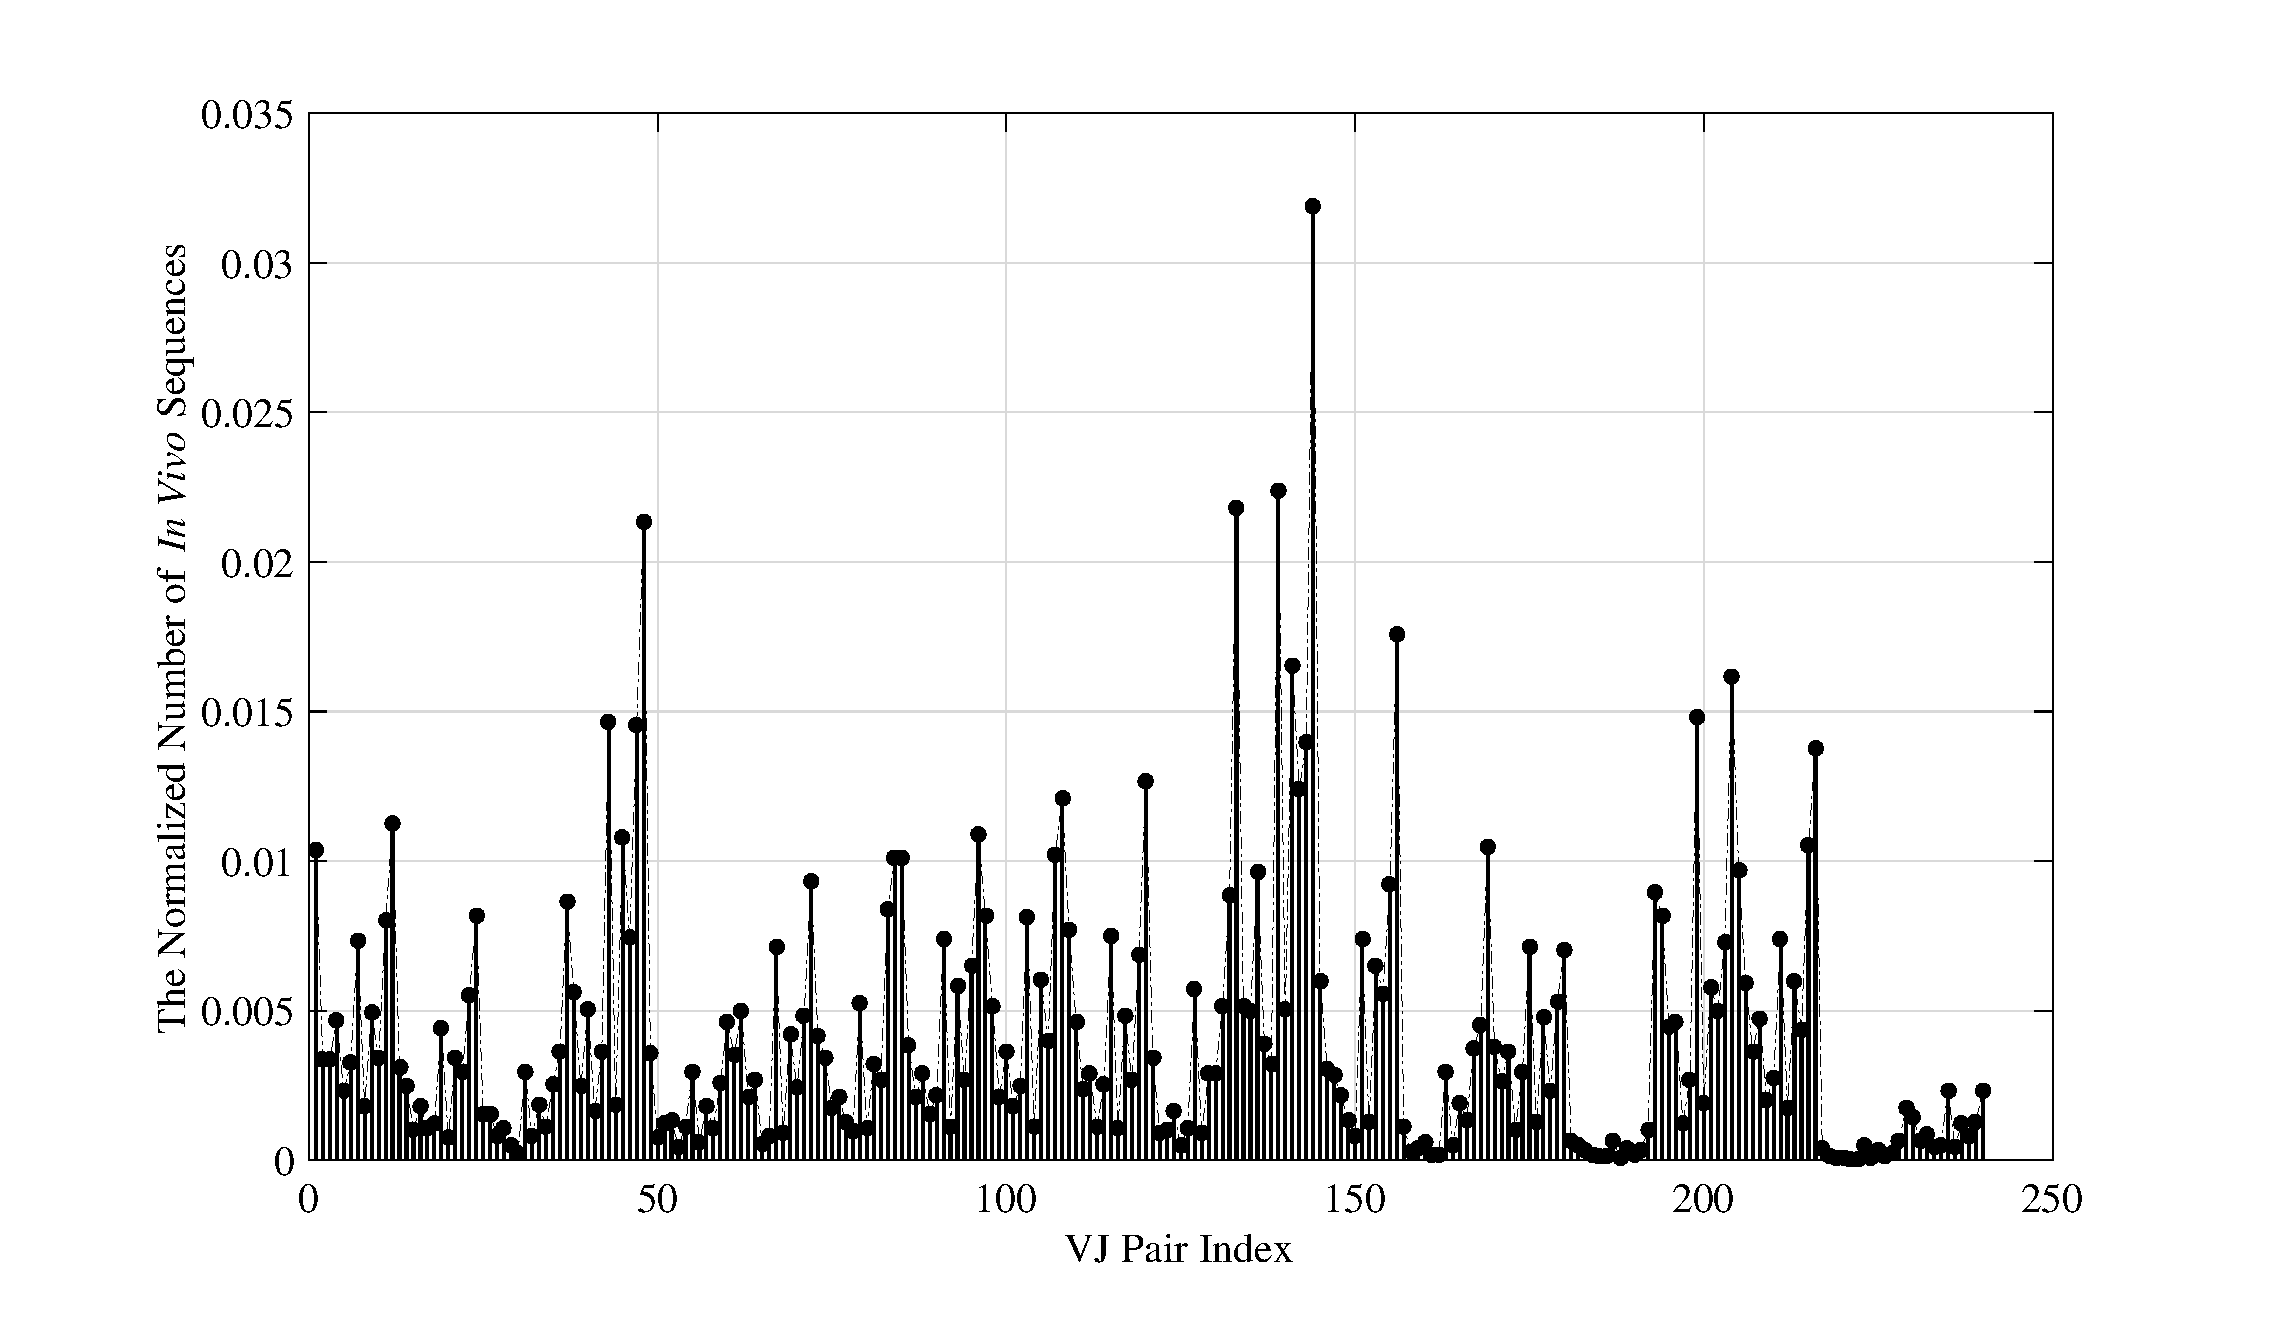
\includegraphics[clip,width=1\columnwidth]{Figure/1.eps}

\caption{ A Normalized distribution of \emph{in vivo} sequences across 240 VJ pairs.}
\label{fig:240PE}
\end{center}
\end{figure}


The second solution would be n-nucleotide level parallelism, where each thread is assigned a unique n-nucleotide sequence and the recombination process is applied on that unique sequence. In this assignment, the workload for the \emph{combination} step is even since, each thread works on one n-nucleotide sequence. In addition, the workload distribution for \emph{comparison} step is equal among GPU threads, since GPU threads are working on the same $V$ and $J$ gene. Therefore, total number of \emph{in vivo} sequence for the comparison process are equal among active threads. Since all threads share the same $V$ and $J$ gene pairs, this approach can take advantage of the shared memory to improve the the memory bandwidth utilization. 

In order to decide which one of the stated approaches performs better in terms of execution time, we evaluate the workload per thread for the \emph{combination} step, in both approaches. In the fine-grained $V-J$ level parallelism, each thread generates \emph{in silico} sequences for all possible forms of n-nuclotide for length of zero to ten. Table \ref{tab:n-table} shows the total number of n-nucleotide sequence based on the length. Therefore, a single thread must generate 706,042,015 \emph{in silico} sequences through the entire process as there are 1,381,717 unique n-nucleotide sequence in total and there are 505 sequences for $D$ gene. In the n-nucleotide based assignment, each thread generates 51,735,230 \emph{in silico} sequences since there are 362 $V$ genes, 283 $J$ genes, and 505 $D$ genes. As a result, workload per thread in fine-grained $V-J$ level parallelism is almost 13 times higher than n-nucleotide parallelization approach. In the following sections we present our approach to bit-wise and multi-GPU implementations based on n-nucleotide level parallelism. 



\begin{table}[t!]
\caption{The total number of unique n-nucleotide sequences based on the length of n-nucleotide}

\renewcommand{\arraystretch}{1.2}
\begin{center}
\begin{tabular}{ |c|c| }
  \hline
    \textbf{\textit{ N\_{len} }} & \textbf{\textit{Total number of unique}}\\
    ~ &  \textbf{\textit{n-nucleotide sequences}}\\	\hline	
    0 & 1  	\\	\hline
    1 & 4 		\\	\hline
   	2 & 16 \\	\hline
    3 & 64 	\\	\hline
    4 & 256 	\\	\hline
    5 & 1,024  	\\	\hline
    6 & 4,096 	\\	\hline
   	7 & 16,384  	\\	\hline
    8 & 65,536 \\	\hline
    9 & 262,144   \\	\hline
    10 & 1,048,576 \\	\hline
    Total & 1,381,717 \\
  \hline
\end{tabular}

  \label{tab:n-table}
\end{center}

\end{table}




\section {The Bit-Wise Implementation }\label{sec:bitwise}
Mainly, there are two phases for the implementation of bit-wise representation. The first phase involves converting the input data set from character domain to binary domain, which we refer to as data conversion phase. The second phase consists of developing GPU kernel using bit-wise operations. We provide detailed explanation regarding the implementation of bit-wise version of the recombination process in the following subsections. 
%The input data set is unique for a given species. For example, human beings have a different set of $V$ and $J$ genes than the mice. 

\subsection {Conversion of input data set}
The main objective of using bit-wise operations for mapping the recombination process is to reduce the memory footprint and execution time. We represent each base (A, C, T, and G) with two bits as shown in Table \ref{tab:encode} and pack a sequence of four bases into a single byte. For those sequences ($V$, $D$, and $J$) whose length is not divisible by four, remainder bases will not fill the byte to its capacity. In this case, we zero pad the end of sequence such that the length of the binary string is divisible by eight (one byte). Let's consider a $V$ sequence, which has the length of ten characters (20 bits). For this case, four zeros are appended to the end of $V$ sequence. As a result, the new $V$ sequence has 24 bits, which requires three bytes of data to store in the memory. The last byte of this $V$ sequence has four zero padded bits, which we refer to as \emph{padded bits}. We call the first two bytes, which only contain the original bits of the $V$ sequence as \emph{full byte}. 

The maximum length of \emph{in vivo} sequences is 60 characters (bytes). In the baseline implementation, \emph{in vivo} sequences are padded with $0$`s so that the length of all sequences are equal to 64 bytes. This guarantees that the allocation of each sequence is equal to the number of threads in two warps, ensuring the memory is aligned to realize coalesced memory accesses. In the binary representation form with 2 bits per base (character), we also follow the same encoding procedure with padding, and represent each \emph{in vivo} sequence with fixed size of 16 bytes.

In the baseline implementation, all possible forms of $V$, $D$, and $J$ sequences are stored in the constant memory to take advantage of the temporal locality it offers. However, the \emph{in vivo} sequences are stored into the GPU's global memory as there are too many \emph{in vivo} sequences ($>$ $10^5$) to fit into the constant memory. For the bit-wise implementation, the \emph{in vivo} data set is also stored in the global memory since the required constant memory for the binary representation of \emph{in vivo} data set is larger than the available constant memory in a target GPU.
%allows us to utilize constant memory alone without having to resort to the global memory.
%We also follow the same memory hierarchy for our design.

\begin{table}[t!]
\caption{2-bit encoding scheme}

\renewcommand{\arraystretch}{1.2}
\begin{center}
\begin{tabular}{ |c|c| }
  \hline
   \textbf{\textit{ Gene base}}  &\textbf{\textit{2-bit representation }}\\	\hline
    A & 00 \\	\hline
    T & 01 \\	\hline
    C & 10 \\	\hline
    G & 11 \\	
  \hline
\end{tabular}

  \label{tab:encode}
\end{center}

\end{table}


\subsection {GPU Kernel}
%The first step for devising a GPU kernel is to determine the parallelization level. As stated in Section \ref{sec: Parallelization Strategy}, we follow the n-way SIMD based implementation that was proposed in \cite{b2} due to its advantages over the $V-J$ level parallelism. In \cite{b2}, 

For the n-nucleotide level parallelism, the total number of threads is set to the total possible combinations for a given n-nucleotide sequence ($4^m$), where $m$ is the length of n-nucleotide sequence. In this case, all active threads can fetch the same input data ($V$, $D$, $J$, and \emph{in vivo}) and each thread can  apply the recombination process over its assigned n-nucleotide. This reduces the number of memory accesses (global and constant) for a specific gene sequence to one among all active threads.


%In \cite{b2}, the n-way SIMD based implementation is proposed where each thread is assigned a unique n-nucleotide sequence and the recombination process is applied on that unique sequence. Therefore, the total number of threads is set to the total possible combinations for a given n-necleotide sequence ($4^m$), where $m$ is the length of n-nucleotide sequence. In this case,  all active threads can fetch the same input data ($V$, $D$, $J$, and \emph{in vivo})  and each thread can  apply the recombination process over its assigned n-nucleotide. This reduces the number of memory accesses (global or constant) for a specific gene sequence to one among all active threads. 

As mentioned earlier, the \emph{in vivo} sequences are partitioned into 240 groups based on the $V$ and $J$ gene used to generate these sequences. This feature was used to pare down the comparison search space in \cite{b2}. Indeed, \emph{in silico} sequences are only compared against the corresponding portion of the \emph{in vivo} data set instead of being compared with the entire data set. We also use this feature in our design. Therefore, our GPU kernel starts its execution by using $V$ and $J$ gene indexes to determine how many and which \emph{in vivo} sequence will be used for the recombination process. Then each thread is assigned a unique n-nucleotide sequence based on the length of \emph{n sequence, thread ID, and block ID}. We propose a function that generates a unique binary n-nucleotide sequence for each thread to guarantee that there is no duplicate n-nucleotide sequence. Algorithm \ref{Algorithm:1} shows the pseudo code for the \emph{task generator} function, which is used to generate a unique binary n-nucleotide sequence. After assigning a unique task to each GPU thread, the recombination process starts on the GPU.


\begin{algorithm}[t]
 \SetKwInOut{Input}{Input}\SetKwInOut{Output}{Output}\SetKwInOut{Init}{Initialization}
 \Input{$threadId$, $blockId$, and $blockDim$ }
 \Output{n-nucleotide sequence}
	$base[4] = \{00,01,10,11\} $\\
	$G_{index}$ = $threadIdx.x + blockIdx.x * blockDim.x$ \\
  \For{$i = 0$ to 3}{
     \For{$j = 0$ to 9 increment by 2}{
		$temp$ = $base$~[$\{G_{index}+ G_{index}/4^{4*i+(j-2/2)}\}\%4]\ll(8-j)$\\
		n-nucleotide[i] $|$= $temp$
	}
}
 \caption{Pseudo code for the \emph{task generator} function which generate a unique n-nucleotide sequence for each thread based on its thread and block indexes.}
\label{Algorithm:1}
%vspace{-.5em}
\end{algorithm}

%
%\begin{figure}[t!]
%\includegraphics[clip,width=1\columnwidth]{Figure/BinaryFunction.jpg}
%\caption{A function which generate a unique n-nucleotide sequence for each thread based on its thread and block indexes.}
%\label{fig:BinaryFunction}
%\end{figure} 



There are four main loops in the GPU kernel. The first \emph{for loop} iterates through each \emph{in vivo} sequence. Upon entering this loop, threads within the block read a single \emph{in vivo} sequence from the global memory into the shared memory. Since, the \emph{in vivo} sequence is shared among all threads within a block, we use \emph{synchthread()} to assure that all threads wait until the memory transaction is completed. 


The second \emph{for loop} iterates through each $V$ sequence in the current $V$ gene set. All threads within a block read the same $V$ sequence from the constant memory, while they work on a different n-nucleotide sequence. We compare the $V$ sequence against the \emph{in vivo} sequence. To accomplish this, we calculate the total number of \emph{full bytes} and \emph{padded bits} for a given $V$ sequence. Then, we iterate through each \emph{full byte} of the $V$ sequence, and compare it with \emph{in vivo} sequence one byte at a time. If there is a mismatch, we terminate the current comparison for all threads and read a new \emph{in vivo} sequence from global memory. Otherwise, we continue on to comparing the last byte of $V$ sequence with the pertinent byte of \emph{in vivo} sequence. In order to accomplish this, we shift the corresponding byte of \emph{in vivo} sequence to the right by the total number of \emph{padded bits}. Accordingly, we shift that byte to the left by the same amount. We will refer to this process as an \emph{alignment process}. Finally, we compare the last byte of $V$ sequence with the aligned byte of \emph{in vivo} sequence. This procedure is shown in step one of Fig. \ref{fig:Compare}. If the $V$ sequence completely matches with the \emph{in vivo} sequence, we proceed to the next loop. Otherwise, we read a new \emph{in vivo} sequence and repeat the process.  


The third loop iterates through each $D$ sequence. There is a difference between this loop (D-loop) and the previous loop (V-loop). The $D$ sequence can cut the n-nulceotide sequence at any position as explained in Chapter \ref{sec:DNA}. Therefore, each thread generates all possible combinations of $nDn'$ sequence for a given $D$ and n-nucleotide sequences. Then, they compare their $nDn'$ sequence with \emph{in vivo} sequence from the last character that was found to be identical to the $V$ sequence in the previous loop. This is accomplished by shifting the \emph{in vivo} sequence to the left by the length of $V$ sequence. The comparison procedure is shown in step two of Fig. \ref{fig:Compare}, and it is the same process as explained in the V-loop. If there is a mismatch between the \emph{in silico} and \emph{in vivo} sequence, then the thread terminates the current comparison, generates a new combination for $nDn'$ sequence, and repeats the process. Otherwise, we continue on to the next loop. It should be noted that, if a thread generates all possible forms of $nDn'$ sequence for a given $D$ and n sequence, then we load new $D$ sequence and repeat the process.

The final loop iterates through each $J$ sequence. In this loop, we first calculate the length of $VnDn'J$ sequence and compare it with the length of \emph{in vivo} sequence. If the length of \emph{in silico} and \emph{in vivo} sequences are not equal, then we terminate the current comparison and load a new $J$ sequence. Otherwise, we compare the $J$ sequence with the latter portion of \emph{in vivo} sequence as shown in step three of Fig. \ref{fig:Compare}. If a sequence generated by a thread matches with the \emph{in vivo} sequence, then that thread increments the local counter stored in a register. A thread may generate the targeted \emph{in vivo} sequence through multiple recombination paths. After all threads complete their n-nucleotide level workload, the counter value stored in the shared memory for that \emph{in vivo} sequence is updated through reduction. At the end of this loop, reduction determines the total number of times an \emph{in vivo} sequence is generated artificially. Finally, the first thread within the block updates the counter value in the global memory.

\begin{figure*}[htbp]
\begin{center}
\includegraphics[clip,width=1\columnwidth]{Figure/Fig.jpg}
\caption{Brief view of the comparison process for the bit-wise version of $V(D)J$ recombination process.}
\label{fig:Compare}
\end{center}
\end{figure*}

\section {The Multi-GPU Implementation} \label{sec:Multi-GPU}
%In this section, we provide a detailed explanation for extending the bit-wise implementation to a multi-GPU environment. 
%There are two steps for a multi-GPU implementation of the recombination process. The first step involves deciding about memory allocations, data communications, and workload distribution among GPUs. The second step consists of performing reduction process to obtain final results from multiple GPUs. 

%As discussed in Section \ref{sec: Parallelization Strategy}, we employ the n-way based parallelization approach for the multi-GPU implementation due to its advantages over the fine-grained $V-J$ level parallelism. 
In n-nucleotide level parallelization, threads of a GPU are assigned a unique n-nucleotide sequence while they work on the same $V$ and $J$ gene. From multi-GPU implementation perspective, in order to generate a unique n-nucleotide sequence for each active thread, we define a global index for each thread based on its thread Id, block Id, GPU Id, and GPU dimension as shown in (\ref{eq:1}) and utilize a \emph{task generator} function that is presented in the algorithm \ref{Algorithm:1}.
\begin{equation}\label{eq:1}
G_{index} = threadIdx + blockIdx \times blockDim + GPUIdx \times GPUDim.
\end{equation}



For the n-nucleotide based parallelization approach, GPU threads work on the same $VJ$ pair so they require accessing the same \emph{in vivo} sequences. Therefore, we replicate input data set and store it in the constant and global memories of each GPU to avoid data transfer between the GPUs.

In order to distribute the workload among GPUs, we first calculate the total number of required threads, which is $4^m$, where $m$ is the length of n-nucleotide sequence. Then, we calculate the total number of required blocks based on the thread-block configuration (refer to Fig. \ref{fig:NormalizedPerf}). Finally, we calculate total number of blocks in each GPU using \ref{eq:2}. For example, we need $262,144$ ($4^9 $) threads for n-nucleotide length of 9. As we will present later in the experimental results, 128 threads per block configuration, which requires 2048 blocks in total  is the desired configuration on a single GPU.  Assuming that we have two GPUs, based on \ref{eq:2}, each GPU is assigned 1024 blocks with 128 threads in each block. In this assignment, the workload distribution among GPUs and GPU threads are equal. 
\begin{equation}\label{eq:2}
\# blocks = \frac{\# total~threads-1}{\# threads~per~block \times \# GPUs+1}
\end{equation}

%Indeed, GPU threads whose global index (Eq. \ref{eq:1}) are greater than $4^m$ (all possible n-nucleotide sequence for length of $m$), will be idle.  We will refer to this during our execution time analysis over the multi-GPU implementation. 

In order to obtain the final result from multiple GPUs, we perform a reduction process. This process accumulates all the results in the root node and copy them to global memory of the host. 

\section{Experimental Setup}
\label{sec:ExptSetup}

\begin{table}
\caption{P100 GPU Streaming Multiprocessor Resources}
\renewcommand{\arraystretch}{1.2}
\begin{center}
\begin{tabular}{ |c|c| }
  \hline
    \textbf{Parameter} & \textbf{Value} \\ \hline
    Compute Capability & $6.0$ \\
    Streaming Multiprocessors (SM) & $56$ \\
    Threads per Warp & $32$  \\
    Maximum Thread Block Size & $1024$ \\
    Maximum Thread Blocks per SM & $32$ \\
    Maximum Warps per SM & $64$  \\
    Maximum Threads per SM & $2048$ \\
    Maximum 32-bit Registers per SM & $65536$ \\
    Maximum Registers per Block & $65536$ \\
    Maximum Registers per Thread & $255$ \\
    Maximum Shared Memory Size per SM & $64$~KB \\
    Constant Memory Size & $64$~KB \\
    \hline
\end{tabular}
  \label{tab:P100params}
\end{center}
\end{table}

We conducted our experiments on a cluster consisting of NVIDIA P100 GPU accelerators. The system is composed of 400 nodes (Intel Haswell V3 28 core processor, 192 GB RAM per node) in which 46 of them are configured as accelerator nodes with a single Nvidia P100 GPU in each node. The cluster uses FDR Infiniband for node to node interconnect and 10 Gb Ethernet for node to storage interconnect. Table \ref{tab:P100params} summarizes the GPU parameters. The P100 GPU has $56$ streaming multiprocessors (SM), each limited to having up to $2048$ threads, $32$ thread blocks, and $64$~KB shared memory. For the bit-wise implementation of the $V(D)J$ recombination algorithm with n-level granularity, each thread utilizes $48$ registers, while there are $65536$ registers available per SM. Therefore, the maximum number of active threads per SM is $1365$ due to the register usage constraint.
Also, it should be noted that the shared memory usage is not the limiting factor for the active threads per SM. As discussed in Section \ref{sec:bitwise}, the shared memory usage per block is $16$ bytes plus one byte per thread for the counter value storage. Thus if we consider block size of 128 threads, only $134$ bytes of shared memory is required per thread block, allowing 489 thread blocks per SM. Given that for n-nucleotide length of nine, there are 2048 blocks for the 128 threads per block configuration. Due to register usage constraint, there are only 10 active thread blocks per SM. As a result, we do not reach the limiting factor (489 thread blocks per SM) for the shared memory usage.

\section {Experimental Results}
\label{sec:Result}

%In this section, we provide a detailed explanation about the experimental setup and the results of the single and multi-GPU implementations. 
We start our analysis by determining the best thread-block configuration for different n-nucleotide lengths on a single GPU. We then compare the execution time of our bit-wise based implementation with the baseline \cite{b2} implementation for each n-nucleotide length. Finally, we present execution time analysis for the multi-GPU implementation with up to eight nodes.

%We should mention that there is a constraint to launch a total of $56\times2048=114,688$ threads in a single P 100 GPU. Since, for bit-wise implementation of the $V(D)J$ recombination process with n-level granularity, each thread utilize 48 register, while there are only $65536$ registers per multiprocessor (MP). Therefore, the maximum number of active thread per SM is 1365. It should be noted that shared memory  does not cuas any constranit as its usage per block is 16 bytes (refer to Section \ref{sec:bitwise}) plus one byte per thread for the counter value storage, a total of 134 Bytes per thread block considering 128 threads per block.  While, P100 GPU has 48 KBytes shared memory per thread block, 64 KBytes shared memory per multiprocessor (MP).


%As mentioned before, the total number of required threads depends on the length of n-nucleotide sequence. For example if the length is eight we need $65,536$, a workload that is mappable to a single GPU. On the other hand for length of nine, we need a total of $4^9 = 262,144$ threads. This workload is expected to benefit from a multi-GPU implementation.
%\vspace{-3 mm}
\subsection {Thread Block Configuration Analysis}\label{subsec:thread}

Fig. \ref{fig:NormalizedPerf} shows the normalized results for  four different thread block configurations over n-nucleotide length ranging from four to ten. For each length of n-nucleotide sequence, we take the shortest execution time and use that as a dividing factor over the execution time of other configurations. Therefore, normalized value of $1$ represents the best performance for a given length. We did not consider n-nucleotide length of zero to three as there are not sufficient threads to utilize multiple \emph{warps} executing concurrently. As shown in Fig. \ref{fig:NormalizedPerf}, there are negligible differences between performance of various thread block configurations for length of four to six since, there are not sufficient tasks to utilize all the available multiprocessors of the P100 GPU. For n-nucleotide length of less than seven, the thread utilization is bellow 14\% as the total number of required threads is less than $2^{14}$ while there are 114,688 threads available in P100. However, for n-nucleotide length of greater than seven, the workload increases such that more than 60\% of available GPU threads are used.
\begin{figure}[t!]
\begin{center}
\includegraphics[clip,width=1\columnwidth]{Figure/Norm_Perf.jpg}

\caption{Normalized results of four different thread per block configurations (32, 64, 128, 256) for n-nucleotide length of four to nine. }
\label{fig:NormalizedPerf}
\end{center}
\end{figure}
There is a 20\% reduction in the performance for the n-nucleotide length of seven based on 256 threads per block configuration compared to other configurations. For n-nucleotide length of seven, the recombination process completes in one iteration for every thread per block configuration since the total number of required threads is $4^7= 16,384$, which is less than the total number of available threads in a single P100 GPU. The lower thread block utilization per SM is the root cause for this performance loss as shown in Table \ref{tab:threadblock}, which reports the thread, thread block, and \emph{warp} utilization for each configuration. 
\begin{table}[t!]
\caption{GPU resource utilization for n-nucleotide length of seven with four different thread block configurations.}

\begin{center}
\begin{tabular}{ |c|c|c|c|}
  \hline
   \textbf{\textit{ thread block }} & \textbf{\textit{threads per SM}} & \textbf{\textit{thread blocks}} & \textbf{\textit{warp}}\\	
   ~ \textbf{\textit{ configuration}} & &\textbf{\textit{ per SM}} & \\ \hline
    32 & 1024 (50\%) & 32 (100\%) & 32 (50\%) \\	\hline
    64 & 1344 (65\%) & 21 (65\%) & 42 (65\%)\\ 	\hline
    128 & 1280 (62.5\%) & 10 (31.25\%) & 40 (62.5\%)\\	\hline
    256 & 1280 (62.5\%) & 5 (15.62\%) & 40 (62.5\%)\\
  \hline
\end{tabular}
\label{tab:threadblock}
\end{center}
\end{table}


We observe a 35\% reduction in the performance for the n-nucleotide length of eight, if 32 threads per block are employed. The reason is that the maximum number of active thread-blocks per multiprocessor is 32 in the P100 GPU. Therefore, we are limited by the hardware to have 32 active blocks per SM in which each block has 32 threads. As a result, we have $2^{10}\times56$ active threads in GPU while we need $2^{16}$ threads to complete the recombination process in one iteration. Let's consider the 64 threads per block configuration, based on the register constraint usage, we can have maximum $1365$ active threads per SM, and based on the thread block configuration, we can have maximum of $21$ blocks with $64$ threads. This results in total of $21\times64\times56=75,264$ threads, which is greater than the required threads for n-nucleotide length of eight. Therefore, the recombination process completes in one iteration for thread block configuration of 64 for n-nucleotide length of eight, while it can not be completed in one iteration with 32 threads per block. We note that the difference between the performance of 64, 128, and 256 threads per block configurations is negligible with normalized values of 1, 0.961, and 0.95 respectively as the recombination process is completed in one iteration for all three configurations.

For n-nucleotide length of nine, the total number of required threads is $4^9= 262,144$, which is greater than available threads in a single GPU. This will results in completing the recombination process in more than one iterations. For 64, 128 and 256 threads per block configurations, four iterations is required to complete the recombination process. As a result, there is a negligible difference between their performances with normalized values of 0.984, 1 and 0.994 respectively. However, the number of required iteration increases by one, if 32 threads are employed per block. Therefore, the poorest performance belongs to 32 thread per block configuration for n-nucleotide length of nine. 

 
In summary, based on  Fig. \ref{fig:NormalizedPerf}, we set thread block configuration to 64 for n-nucleotide lengths four to eight, 128 for lengths nine and ten. In the following subsection, we evaluate the performance of bit-wise and multi-GPU implementations with respect to the the baseline implementation. 


\subsection {Bit-wise Simulation Results}
In order to evaluate the bit-wise implementation, we ran an experiment on a single Tesla P100 GPU using the baseline implementation. The timing analysis and memory footprint for this experiment are used as a reference point for performance comparison.  

Table \ref{tab:bit-wise-mem} shows the total amount of required memory for $V$, $D$, $J$ genes, and \emph{in vivo} data set using the bit-wise representation. As stated in table \ref{tab:bit-wise-mem}, the memory footprint for constant memory reduces by a factor of 3.4 compared to the baseline implementation, while the required global memory reduces by a factor of 4. Table \ref{tab:bit-wise-time} shows the execution time results for each n-nucleotide length. Last row shows the total execution time for the recombination process.  As shown, the total execution time reduces by a factor of 2.1 in comparison with the baseline implementation. 
For both implementations, after n-nucleotide of eight, the execution time increases by about a factor of four at each increments of n-nucleotide length by one. For n-nucleotide length of eight, we utilize  87.5\% of available SM on a single GPU since 49 MPs with thread block configuration of 64 (smallest execution time) are used. Therefore, increasing the workload beyond this point directly results in increasing the execution time. The workload per GPU depends on the total number of unique n-nucleotide sequence as mentioned in \ref{sec: Parallelization Strategy}. Therefore, increasing the length of n-nucloetide by one results in increasing the total number of unique n-nucleotide sequences by a factor of four and as a result execution time increases with the same factor.   

\begin{table}[t!]
\caption{The memory footprint for the bit-wise implementation in comparison with the baseline approach.}

\renewcommand{\arraystretch}{1.2}
\begin{center}
\begin{tabular}{ |c|c|c|c| }
  \hline
    \textbf{\textit{}}  & \textbf{\textit{}}  & \textbf{\textit{}} & \textbf{\textit{Percentage}}\\	
    \textbf{\textit{Gene}} & \textbf{\textit{Baseline \cite{b2}}}& \textbf{\textit{Bit-wise}}& \textbf{\textit{ reduction}}\\ \hline
    $V$ & 1448 & 425  & 70.65 \\	\hline
    $J$& 3107 & 913  & 70.61\\ 	\hline
    $D$& 3210  & 908  & 71.71\\	\hline
    \emph{in vivo}& 6517568  & 1629392  & 75.00 \\	 
    %Constant memory & 7765 & 2246  & 71.07\\ \hline
    %Global memory & 6517568  & 1629392  & 75.00 \\
  \hline
\end{tabular}
  \label{tab:bit-wise-mem}
\end{center}

\end{table}

\begin{table}[t!]
\caption{Execution time on single GPU: Baseline vs. Bit-wise Implementations }

\renewcommand{\arraystretch}{1.2}
\begin{center}
\begin{tabular}{ |c|c|c| }
  \hline
   \textbf{\textit{ \emph{N} length }} & \textbf{\textit{Baseline (min)}} & \textbf{\textit{Bit-wise (min)}} \\	\hline
    0 & 8.36 & 8.68 \\	\hline
    1 & 10.17 & 9.34 \\ 	\hline
    2 & 12.57 & 10.14\\	\hline
    3 & 15.38 & 10.92 \\	\hline
    4 & 18.47 & 11.74\\	\hline
    5 & 21.73 & 12.56\\ 	\hline
    6 & 25.67 & 13.69\\	\hline
    7 & 32.09 & 16.23\\	\hline
    8 & 102.03 & 49.82\\	\hline
    9 & 426.9 & 196.76\\		\hline
    10 & 1755.35 & 797.8\\	\hline
    Total & 2428.7 & 1137.7 \\
  \hline
\end{tabular}
  \label{tab:bit-wise-time}
\end{center}
\end{table}

\subsection {Multi-GPU Simulation Results}
Table \ref{tab:multi-gpu-time} shows the  execution time of the multi-GPU version of the bit-wise implementation for each n-nucleotide length. We ran experiments by using up to eight GPUs to evaluate the trends in execution time improvement with respect to change in number of GPUs. 

The key observation from Table \ref{tab:multi-gpu-time} is that there is slight increase in execution time if multiple GPUs are utilized for n-nucleotide length less than eight. The reason behind this observation is the fact that the P100 GPU is over-provisioned; the total number of required threads for any n-nucleotide length less than eight are less than the maximum $2048\times56 = 57,344)$ active threads. Moreover, the extra reduction step for a multi-GPU implementation becomes a slight overhead.

\begin{sidewaystable}
    \centering
%\begin{table}
\caption{Execution Time for the bit-wise implementation on different number of GPUs.}

%\begin{center}
\scalebox{0.7}{
\begin{tabular}{ |c|c|c|c|c|c|c|c|c|}
  \hline
   \textbf{\textit{ N length }} & \textbf{\textit{1-GPU (min)}} & \textbf{\textit{2-GPUs (min)}} & \textbf{\textit{3-GPUs (min)}} & \textbf{\textit{4-GPUs (min)}} & \textbf{\textit{5-GPUs (min)}} & \textbf{\textit{6-GPUs (min) }}& \textbf{\textit{7-GPUs (min)}} & \textbf{\textit{8-GPUs (min)}}\\	\hline
    0 & 8.68 & 9.23 & 9.28 & 9.09 & 9.09 & 9.09 & 9.1 & 9.09\\	\hline
    1 & 9.34 & 9.91 & 9.97 & 9.77 & 9.77& 9.78 & 9.78 & 9.78\\ 	\hline
    2 & 10.14 & 10.69 & 10.75 & 10.55 & 10.56& 10.56 & 10.55 & 10.56\\	\hline
    3 & 10.92 & 11.48 & 11.55 & 11.34 & 11.35& 11.35 & 11.35 & 11.35\\	\hline
    4 & 11.74 & 12.29 & 12.37 & 12.12 & 12.13& 12.12 & 12.13 & 12.12\\	\hline
    5 & 12.56 & 13.18 & 13.24 & 13.03 & 13.03& 13.01 & 13.01 & 12.97\\ 	\hline
    6 & 13.69 & 14.34 & 14.39 & 13.91 & 13.90 & 13.90 & 13.89 &13.88\\	\hline
    7 & \cellcolor{blue!25}16.23 & 16.61 & 15.66 & 15.43 & 15.32 & 15.28 & 15.26 &15.23\\	\hline
    8 & \cellcolor{green!25}49.82 & 27.89 & 22.77 & \cellcolor{blue!25}18.92 & 17.62& 17.57 & 17.55 & 17.52\\	\hline
    9 &\cellcolor{pink!25} 196.76 & 112.86 & 82.00 & \cellcolor{green!25}58.60 & 46.59& 40.22 & 34.36 & 28.70\\		\hline
    10 & 797.8 & 455.73& 301.18 & \cellcolor{pink!25}231.37 & 185.31 & 159.48 & 139.62 & 116.22\\	\hline
    Total & 1137.7 & 694.21& 513.16 & 404.13& 344.67& 312.36 & 286.6& 257.42\\
  \hline
\end{tabular}
\label{tab:multi-gpu-time}
%\end{center}
}
%\end{table}
\end{sidewaystable}

However, for n-nucleotide length more than seven, we observe a reduction in the execution time with multiple GPUs. This is due to the fact that a single GPU is almost fully utilized at 87.5\% as explained in Section \ref{subsec:thread} for n-nucleotide length of more than seven. Since the required number of threads exceeds the active thread count per GPU, we observe the benefit of the multi-GPU implementation for n-nucleotide length eight and above. At this point, we expect to see relatively linear reduction in the execution time for a given n-nucleotide length as we increase the number GPUs. However, the simulation results show a saturating execution time trend where adding another GPU resource no longer helps reduce the execution time. We further investigate this behavior in the following paragraph.

%{\color{red} please writ trend analysis for 8. this is good as we see clear saturation at 4 GPU. we don't se that in nine. this requires more GPUs}
 
For n-nucleotide length of nine, the required number of threads is $4^9= 262,144$, which is more than the available threads in a single P100 GPU. Based on the register resource constraint, the recombination process can be completed in four iterations ($\lceil(4^9/1280\times56)\rceil=4 $) using a single GPU. In this case there are $47,104$ active threads in the last iteration utilizing 65\% of the GPU threads. Employing two GPUs results in completing the process in two iterations, while there are $32,768$ threads in the last iteration. In this case we are only utilizing 45\% of the GPU threads. Therefore, we do not observe two times speed up with two GPUs. 
Utilizing four GPUs for n-nucleotide length of nine results with completing the process in one iteration. Beyond this point, increasing the number of GPUs causes under-utilization of each GPU and does not significantly improve the execution time.  

%Hence, using two GPUs reduces the execution time by 1.786$\times$, but as we increase number of GPUs the execution time improvement per GPU reduces because of the GPU under-utilization and nature of the $V(D)J$ recombination process which we discuss in the following.

For n-nucleotide length of ten, the required number of threads is $4^{10}=1,048,576$.  The recombination process is completed in 15 iterations ($\lceil(4^{10}/1280\times56)\rceil=15 $) using a single GPU while there are $45056$ active threads in the last iteration (62\% GPU threads utilization). However, employing two GPUs results in completing the process in 8 iterations.  The reduction of execution time from 797 minutes to 455 minutes is proportional to the reduction of iteration count from 15 to 8, which is the root cause for not observing a linear speedup with two GPUs. Using three GPUs results in completing the recombination process in 5 iterations while the GPU thread utilization is at 87.6\% in the last iteration. When we employ four GPUs, iteration cont becomes 4. For the GPU count of five, six, and seven, the iteration count remains at 3 with fewer threads being utilized as the number of GPUs increases.  In order to complete the process in one iteration, we need to employ 16 GPUs. In overall, the saturation in the reduction of iteration count as we increase the GPU resources combined with the under utilization of the threads during the last iteration of the recombination process are the two root causes of saturating trend in execution time with respect to GPU count. 


For the single GPU version, in the previous section, we showed that execution time increased by about a factor of four at each increments of the n-nucleotide length. Since we distribute the workload equally across the GPUs, we observe  a similar  trend for the multi-GPU implementation. For example, as shown in Table \ref{tab:multi-gpu-time}   execution time using two GPUs for n-nucleotide length of nine is about four times the execution time for n-nucleotide length of eight. Consistently we observe about a factor of four as we increase length from nine to ten for all GPU configurations. 

Furthermore, we should expect the same execution time for two consecutive n-nucleotide lengths, while using one GPU for the first one and using four GPUs for the second one. As highlighted in Table \ref{tab:multi-gpu-time}, the execution time for n-nucleotide length of nine is 196 minutes by using single GPU. However we observe that execution time is 231 minutes for n-nucleotide of ten with four GPUs. We identify factors to this discrepancy as overhead of reduction process with the increase in number of GPUs, difference between the total number of $nDn'$ combinations, and difference between the number of times each thread finds a match or terminates early. As stated earlier in Chapter \ref{sec:DNA}, the $D$ sequence can cut n-nucleotide sequence at any position, and each thread needs to generate all possible combinations of $D$ with n-nucleotide sequence. As the length of n-nucleotide increases, the total possible combinations of $nDn'$ increases by one for given $D$ and n-nucleotide sequences. We note that an extra sequence needs to be combined with all possible forms of $V$ and $J$ gene sequences, which explains the difference between what we expected and what we observed. The difference in execution time reduces to around 9 minutes between n-nucleotide length eight with a single GPU and n-nucleotide length of nine with 4 GPUs. This discrepancy is about 2.6 minutes for the length pair of seven and eight with 1 and 4 GPUs respectively. We attribute this discrepancy reduction trend to the three factors listed above. 
  

\chapter{FPGA-based Implementation of The DNA Recombination Algorithm\label{chapter:FPGA}}
In this Chapter, we study the implementation of $V(D)J$ recombination process on FPGA using the n-necleotide level parallelism that was used in the GPU-based implementation in Section \ref{sec:N-level}. As we converge to a final hardware architecture, we provide a detailed explanation for each unit individually. We explain the experimental results for the n-level FPGA-based implementation of $V(D)J$ recombination process in Section \ref{sec:simNlevel}. Based on the simulation results, we explain the draw back of n-level paralleization method for FPGA-based implementation of the recombination process in Section \ref{sec:drawbackNlevel}. As a result, we proposed the VJ level parallelization approach for the FPGA-based implementation to overcome the draw back of n-level approach in Section \ref{sec:VJ level}. We describe the structure of each unit of the final hardware architecture for the VJ method. Finally, we describe the simulation results for the new parallelization approach in Section \ref{sec:simVJlevel}. 



\section{Hardware Implementation of N Level Parallelization }\label{sec:N-level}

The goal for the hardware implementation of DNA recombination process is to accelerate the generation of all possible TCR sequences with any given $V$, $D$ and $J$ gene sequences and count the number of times each sequence can be generated artificially. As we converge to a final hardware architecture for this process we need to determine the level of parallelism and granularity of the processing elements for generating \emph{in silico} sequences, orchestrate the data transfers between the memory  and computation units, and balance the trade-off between throughput and resource usage. In this section, we first  describe the parallelization strategy and then explain the structure of each unit that is used to implement the $V(D)J$ recombination algorithm.
%individually in Section \ref{subsec:Parallel}. 
%Second, we provide a detailed explanation for the structure of input data set in section \ref{subsec:dataset}. 
%Then, we explain the structure of each unit individually in Subsections \ref{subsec:processing unit} - \ref{AGU}. 

Fig \ref{fig:BIG-Picture_NLevel} shows the proposed architecture for the hardware implementation of the recombination process, which consists of three units, address generator unit (AGU), memory bank unit, and  processing unit. The processing unit (PU) consists of processing element (PE), n-sequence initiator, and \emph{in vivo} address generator units. The PE consists of a number of parallel computation units (CUs), which is formed of concatenation and comparison units.   

The PU generates the number of times  each \emph{in vivo} sequence can be generated artificially in cooperation with the memory bank unit and corresponds to the inner most three loops in Algorithm \ref{Algorithm:2}. The n-sequence initiator provides the legitimate n-nucleotide length and reference n-nucleotide sequence for each CU based on the length of each input  $V$, $D$ and $J$ gene sequences. Each CU  generates a unique  n-nucleotide sequence, forms all possible  \emph{in silico} sequences based on  the input $V$, $D$ and $J$ gene sequences,  and searches those generated sequences in the \emph{in vivo} memory bank. The \emph{in vivo} address generator unit allows reading the \emph{in vivo} sequences and their counter values for each CU, and updates the counter value when a match is found by a CU. The AGU is corresponds to the outer most three for loops in Algorithm \ref{Algorithm:2} in order to generate the indexes for accessing the $V$, $D$, $J$ sequences.  The memory bank unit is compromised of four sub-memory banks for maintaining input and output data sets. 



\begin{figure}[t!]
\begin{center}
\includegraphics[clip,width=1\columnwidth]{Fig/BIG-Picture_NLevel.jpg}
\caption{The hardware implementation of $V(D)J$ recombination process using the N-level parallelization approach.}
\label{fig:BIG-Picture_NLevel}
\end{center}
\end{figure}

\subsection{N Level Parallelization Strategy}\label{subsec:Parallel}

In this section, we present a series of experimental analysis to answer the following four questions that will help us determine the degree of parallelism ($D_{p}$) to realize in the final architecture:

1) What is the efficient parallelization strategy that will minimize the execution time, 
2) How does the workload partitioning strategy across the CUs affect the performance based on the resource constraints imposed by the target FPGA,
3) What is the correlation of the $D_p$ with the resource utilization and the critical path delay, and
4) How does the $D_p$ affect the throughput?

As mentioned in Chapter \ref{sec:DNA}, all possible forms of n-nucleotide sequences are involved in the recombination process. The length of n-nucleotide ($N_{length}$) can be between zero to ten and the n-nucleotide sequence can be placed on either side of $D$ sequence. Table \ref{tab:1} shows the total number of unique n-nucleotide sequences based on the $N_{length}$ along with the total number of possible combinations of $n_{1}$D$n_{2}$ with a given $D$ sequence given that $D$ gene can partition the n-nucleotide of  size $N_{length}$ at any position generating $N_{length}+1$ such partitioning opportunities. Therefore, if the length of $D$ sequence is greater than zero then, the total possible combinations is equal to $4^{ N_{length}} \times (N_{length}+1)$.

The computation requirement is the same for generating  the \emph{in silico} sequences based on each of the $4^{ N_{length}}$ unique n-nucleotide sequences. This creates an opportunity to parallelize at n-nucleotide level and achieve a balanced workload distribution across the computation units. This was the parallelization approach taken in our GPU-based implementation to achieve a balance workload across the threads and thread blocks of the GPU.  
Consider the case of $N_{length}$ of ten, which generates over one million unique sequences. Hardware implementation at a scale of million CUs is not feasible due to  the resource constraints. Therefore a partial parallelization is needed and the resource demand for a single CU helps us determine the amount of unrolling we can apply to the loop with index four in Algorithm \ref{Algorithm:2} and derive the number of CUs we can instantiate on the target FPGA. This number will also help us determine the structure of the n-sequence initiator and PU. Therefore, in order to answer the second question, we implement a single CU, that is composed of concatenation and comparison units on the the Virtex-7 XC7VX485T FPGA. We will describe the details of the PU structure in section \ref{subsec:processing unit}. As shown in table \ref{tab:2}, the "Slice LUTs" is the determining factor and we can fit up to 256 CUs leaving 15\% of the resources for the AGU state machine, $n-$sequence initiator unit, \emph{in vivo} address generator and glue logic. 

In order to answer the third question, we implement the proposed architecture for different $D_p$ and plot the resource utilization trend as shown in Fig. \ref{fig:ResourceUtil}. As we increase the $D_p$, the resource utilization increases linearly. We show the critical path delay with respect to changes in $D_p$  in Fig. \ref{fig:CriticalPath} to answer the third question. As shown, the critical path delay slightly increases as the $D_p$ increase. 

In order to answer the last question, we first need to define the throughput. The throughput is defined as the total number of comparisons per second. Since, we have the same number of comparison units as the $D_P$, the throughput increases linearly.

Based on the above analysis, we set the $D_P$ equal to 256 and the final architecture based on our n-nucleotide level parallelization strategy is shown in Fig. \ref{fig:BIG-Picture_NLevel}. In the following sections, we explain the structure of each unit within the processing core (PC) in detail.

\begin{table}[t!]
\caption{The total number of unique n-nucleotide sequences and total number of possible combinations of  $n_1$D$n_2$ with a given $D$ sequence based on the length of n-nucleotide.}
\begin{center}
\begin{tabular}{ |c|c|c| }
  \hline
    \textbf{\textit{$N_{length}$}} & \textbf{\textit{Total number of unique}} & \textbf{\textit{Total number of possible}}\\
    ~ &  \textbf{\textit{$n-nucleotide$ sequences}} & \textbf{\textit{combinations of $n_1$D$n_2$}}\\
    ~&~& \textbf{\textit{with a given D }}\\ \hline	
    0 & 1  	& 4	\\	\hline
    1 & 4 	& 8	\\	\hline
   	2 & 16 	& 48\\	\hline
    3 & 64 	& 256	\\	\hline
    4 & 256 & 1280	\\	\hline
    5 & 1024 &6144 	\\	\hline
    6 & 4096 & 28672	\\	\hline
   	7 & 16384 &131072 	\\	\hline
    8 & 65536 &	589824\\	\hline
    9 & 262144  &2621440 \\	\hline
    10 & 1048576 & 11534336\\
  \hline
\end{tabular}

  \label{tab:1}
\end{center}
\end{table}

\begin{table}[t!]
\caption{Resource Utilization for a single CU}
\begin{center}
\begin{tabular}{ |c|c| }
  \hline
    Slice LUTs (303600) & 977 \\	\hline
    Slice Registers (607200) & 509\\	\hline
    Slice (75900) & 275	\\hline
    LUT as Logic (303600)& 977\\	\hline
    LUT Flip Flop Pairs (303600) & 272\\
  \hline
\end{tabular}

  \label{tab:2}
\end{center}
\end{table}

\begin{figure}[t!]
\begin{center}
\includegraphics[clip,width=1\linewidth]{Fig/Chart.png}
\caption{The resource utilization of the N-level architecture for different values of the $D_P$. }
\label{fig:ResourceUtil}
\end{center}
\end{figure}



\begin{figure}[t!]
\begin{center}
\includegraphics[clip,width=1\linewidth]{Fig/CriticalPathDelay_ParallelizationLevel.png}
\caption{The critical path delay of the N-level architecture for different values of the $D_P$. }
\label{fig:CriticalPath}
\end{center}
\end{figure}
%\subsection{Input Data Sets}\label{subsec:dataset}
%%%%%%%%%%%%%%%%%%%%%%%%%%%
%The input data sets consist of $V$, $D$, $J$ and \emph{in vivo} genes. In C57BL/6 mice, there are 20 basic $V \beta$ genes, 2 $D \beta$ genes and 12 basic $J \beta$ genes. However, all possible patterns such as chewback and palindromic forms for each of the functional $V$, $D$ and $J$ gene sequences need to participate in the recombination process for modeling the TCR repertoire as illustrated in  Fig\ref{fig:VDJ}. 
%For example, the first basic $V$ gene has a length of 14. For the $V$ gene, up to four genes can be appended to the right end of the $V$ gene from its mirror strand (step one, indicated as +4, +3, +2, +1), therefore the actual length of this gene can be up to 18. This would result with 18 different sequences based on the chewback process (step two). $D$ and $J$ gene data sets go through similar process as explained in section \ref{subsec:Bio}, therefore each $V$, $D$ and $J$ gene data set consists of several forms of sequences with different lengths. In C57BL/6 mice, the \emph{in vivo} data set involves 101822 sequences, which are grouped based on the specific $VJ$ pair used to generate that sequence. There is no other recombination path for an \emph{in vivo} sequence other than the specific $VJ$ pair, which generates that specific sequence. This is a key feature that we will exploit to reduce a search space for the \emph{in vivo} address generator unit and reduce the execution time . There are 240 such pairs since we have 20 basic $V$ genes and 12 basic $J$ genes in mice.



%%%%%%%%%%%%%%%%%%%%%%%%%%%%%%%%%%%%%%%
\subsection{Processing Unit}\label{subsec:processing unit}
%%%%%%%%%%%%%%%%%%%%%%%%%%%%%%%%%%%%%%

As illustrated in Algorithm \ref{Algorithm:2}, modeling the TCRs repertoire involves six nested for loops. We map the inner most three for loops with index 4-6 to the PU to iterate through all possible forms of n-nucleotide additions, create \emph{in silico} sequences, and search for a match of the \emph{in silico} sequence within the \emph{in vivo} data set. We describe the structure of the PU composed of the PE, $n$-sequence initiator, and \emph{in vivo} address generator units in the following subsections.

The inputs to the PU are the $V$, $D$, $J$, and \emph{in vivo} sequences received from their respective memory bank units, the counter received from the conuter memory bank unit, and the VJ group ($group_{id}$) from the AGU. The addresses for these three sequences are determined by the AGU, which will be discussed later. We set the bitwidth for each sequence to 64 as shown in Fig. \ref{fig:BIG-Picture_NLevel}. In C57BL/6 mice data set, the maximum length of the  $V$, $J$ and $D$ gene sequences is 26 characters. We assign two bits to represent each of the four types of nucleotide bases (A, G, C, and T). We reserve five bits to keep track of the length of each sequence. The n-sequence initiator unit will rely on this length information for selecting valid length for the n-nucleotide sequence. In addition, the concatenation unit depends on the length information for generating the \emph{in silico} sequence. As explained earlier in Chapter \ref{sec:DNA}, the $D$ gene goes through chewback process on its both ends. Based on the C57BL/6 mice data set, there are maximum of 22 different paths to generate $D$ sequences. We reserve five bits to represent each path, which we refer to as $D_{Path}$. The \emph{in vivo} address generator unit will require this information for counter update, which will be discussed later. Therefore, in total we need to form a 62 bit package as an input to the PU, however we set the package size as 64 leaving 2-bit  for debugging purpose to set as used or not used.  
 
%%%%%%%%%%%%%%%%%%%%%%%%%%%%%%%%%%%%%%%
\subsection{n-sequence Initiator Unit }\label{subsec:nsequence}
%%%%%%%%%%%%%%%%%%%%%%%%%%%%%%%%%%%%%%
The input to the n-sequence initiator unit are the length of $V$, $D$, and $J$ gene sequences received from their respective memory bank units, the $Request Data$ signal received from the PE. The outputs of this unit are the $Data Ready$, $N_{length}$, length of \emph{in silico} sequence ($sequence_{length}$), and the reference n-nucleotide sequence ($Initial_N$) for the CUs, and $Data Ready$ and $sequence_{length}$ for the \emph{in vivo} address generator unit. We set the bitwidth of $N_{length}$ and $Initial_N$ to five and 20 respectively, as the maximum length of n-nucelotide is 20 bits (ten characters). Also, we set the bitwidth of $sequence_{length}$ to seven as the maximum value for $sequence_{length}$ is 120 bits (60 characters).  

The n-sequence initiator unit implements the for loop indexed  as four in the Algorithm \ref{Algorithm:2}. This loop iterates through n-nucleotide of length zero through ten and generates all possible sequences for that length. We can extend the for loop with index of four into three sub-for loops as shown in Algorithm \ref{Algorithm:1}. 

The first for loop iterates through all possible n-nucleotide sequences of $N_{length}$ between zero and ten. However, all possible n-nucleotide sequences for each length will not result with valid \emph{in silico} sequence based on the given $V$, $D$ and $J$ gene sequences as the $sequence_{length}$ must be within the range of six to sixty characters and divisible by three. Therefore, primary functionality of the n-sequence initiator unit is selecting the legitimate $N_{length}$ and proceed to the next loop. The second for loop iterates through all possible unique n-nucleotide sequences for the selected $N_{length}$. Table \ref{tab:1} shows the total number possible unique n-nucleotide sequences with different length. 

Rather than having this unit generate a n-nucleotide sequence for each CU, and send all possible combinations in rounds each with 256 sequences (as there are 256 parallel CUs), we send only $Initial_N$ as a reference starting address to all CUs and have each CU calculate its unique n-nucleotide sequence using $Initial_N + CU_{id}$, expression where $CU_{id}$ is the index of CU. This allows us to reduce the amount of data transfer to the CUs and wiring requirement on the implementation. After each round, the $Initial_N$ is incremented by 256 to complete all the rounds needed for that specific $N_{length}$, which is  $4^{N_{length}}/256$. The third for loop iterates through all possible combinations for the length of  $n_1$ and $n_2$ sequences to cover all forms of $n_1$D$n_2$ sequence. 

\begin{algorithm}[t]
 
\nl \For{$i = 0$ to 10}{
		\emph{$N_{length}$} = i;
		
		$sequence_{length}$ = $V_{len}$+ $J_{len}$ + $D_{len}$ + $N_{length}$;
		
		\If{$(6<=sequence_{length}<=60)~\&~(sequence_{length} \% 3 == 0)$ }{
			
			\nl     \For{$k = 0$ to $4^i$}{
		
		$Initial_N$ = $k$;
		
		\nl     \For{$j = i$ to 0}{

		$len_{n_{1}}$ = j;
		
		$len_{n_{2}}$ = i-j;
		}
		$k$ = $k$ + $D_P$;
  
}
		}
		

}
 \caption{Pseudo code for expanding the for loop with index of four in Algorithm \ref{Algorithm:2}. }
\label{Algorithm:1}
%vspace{-.5em}
\end{algorithm}


%%%%%%%%%%%%%%%%%%%%%%%%%%%%%%%%%%%%%%%
\subsection{In vivo Address Generator Unit }\label{subsec:InVivoAGU}
%%%%%%%%%%%%%%%%%%%%%%%%%%%%%%%%%%%%%%
The inputs for the \emph{in vivo} address generator unit are the $sequence_{length}$ and $Data Ready$ from the n-sequence initiator, the $group_{id}$ from the AGU, the $Match$ signal indicates that there is a match between \emph{in vivo} and \emph{in silico} sequences, from the $PE$, and the 16-bit counter indicating the number of times that the specific \emph{in vivo} sequence is generated, from the counter memory bank. The outputs are the address for reading the sequence from the \emph{in vivo} memory bank ($in~vivo\_Add$) along with its read enable signal ($in~vivo\_En$) and the address for the sequence's counter value in the counter memory bank ($Counter\_Add$) along with read enable ($Counter\_En$) and write enable ($Counter\_Wr\_En$) signals to control reads and writes. We set the bitwidth of $Counter\_Add$ and $in~vivo\_Add$ to 12 as there are maximum $3249$ \emph{in vivo} sequences in the BRAMs. In addition, we set the bitwidth of $in~vivo\_En$ and $Counter\_En$ to 8 as there are 240 BRAMs in the \emph{in vivo} and counter memory bank units.

Before we describe the functionality of the \emph{in vivo} address generator unit, we need to explain the structure of the \emph{in vivo} memory bank. As mentioned in Section \ref{subsec:input}, the \emph{in vivo} sequences are grouped based on the $VJ$ pair used to generate that sequence. We benefit from this feature to reduce the comparison search space. Therefore, we distribute the \emph{in vivo} data set based on the $VJ$ group assignment across 240 BRAMs, where each BRAM holds  \emph{in vivo} sequences sorted in ascending order of length for that $VJ$ group. This way of data organization allows us to use the $group_{id}$ to search for the data only in one of the 240 BRAMs, and $sequence_{length}$ to search within a single BRAM among the sequences that have the same length. In order to realize this, we need to know the starting and ending addresses of the \emph{in vivo} sequences in the \emph{in vivo} memory bank for any given $sequence_{length}$. Therefore, we utilize two $240$x$19$ arrays ($starting_{array}$, $ending_{array}$), which keep the starting and ending address of \emph{in vivo} sequences for each $sequence_{length}$ and $group_{id}$. The size of $starting_{array}$, $ending_{array}$ is defined based on the total number of $VJ$ groups (240 $VJ$ groups) and the total number of available length for the \emph{in vivo} sequence (19 different lengths from six to sixty characters).
%
%\emph{Step 1:} In this step, we check the status of the $n-$ sequence generator unit. If it has a valid data then, we continue to the next step to calculate the address for \emph{in vivo} memory bank. Otherwise, we remain in this step for the valid data from the $n-$ sequence generator unit.
%
%\emph{Step 2:} In this step, we first calculate the index of $starting_{array}$ and $ending_{array}$ based on $group_{id}$ and $sequence_{lenght}$ using the equation \ref{eq:3}. Accordingly, we can access to the starting address and ending address of \emph{in vivo} memory using the calculated index. Finally, we set the address of \emph{in vivo} memory bank to the starting address and proceed to the next step.
%
%\begin{equation}\label{eq:3}
%Index_{array} = group_{id} \times 12 + \frac{sequence_{length}} {3} - 2	
%\end{equation} 
%\emph{Step 3:} In this step, we read the \emph{in vivo} sequence from the \emph{in vivo} memory bank and pass the \emph{in vivo} sequence to the CUs. Then,we wait for the comparison result from the CUs. If one of the CUs finds a match between the \emph{in silico} and \emph{in vivo} sequences, then we continue on to the fourth step for counter update. Otherwise, we move on to the step five to read new \emph{in vivo} sequence from memory bank.
%
%\emph{Step 4:} In this step, we set the address of counter memory bank to the current address of \emph{in vivo} and read the \emph{counter} from the counter memory bank. Then, we update the \emph{counter} value with the $D_{path}$ and write the updated \emph{counter}  into the counter memory bank. At this point, if we find a match for all of the \emph{in silico} sequences,  then we move to the first step. Otherwise we continue on to the step five to do the comparison between the current address of \emph{in vivo} memory bank and the ending address.
%
%\emph{Step 5:} We compare the current address of \emph{in vivo} memory bank with the ending address of \emph{in vivo} memory bank that is determined in the second step. If it is match, then we go to the first step. Otherwise, we increment the current address  of \emph{in vivo} memory bank by one, and move on to the third step.
%%%%%%%%%%%%%%%%%%%%%%%%%%%%%%%%%%%%%%%
\subsection{Processing Element }\label{subsec:PE}
%%%%%%%%%%%%%%%%%%%%%%%%%%%%%%%%%%%%%%
The inputs for the PE are the $V$, $D$ and $J$ gene sequences from the memory banks, the $sequence_{length}$, $N_{length}$, $Data Ready$ and $Initial_N$  from the n-sequence initiator unit and 128-bit \emph{in vivo} sequence from the \emph{in vivo} memory bank unit. The output is the $Match$ signal for the \emph{in vivo} address generator unit indicating that one of the 256 CUs generated the  \emph{in vivo} sequence. This $Match$ signal triggers the \emph{in vivo} AGU to update the corresponding counter for that  \emph{in vivo} sequence. As shown in Fig. \ref{fig:BIG-Picture_NLevel}, the PE consists of 256 parallel CUs where, each CU consists of a pair of concatenation and comparison units.


The concatenation unit uses an \emph{or} gate to concatenate the $V$, $n_1$, $D$, $n_2$ and $J$ sequences in the given order to form a 128-bit sequence. The position of each sequence in the 128-bit package is determined by the length of the remaining four sequences. This position value is used as the shift amount to apply to each sequence before the $or$ gate based concatenation. We pass the \emph{in silico} sequence to the comparison unit of each CU to compare the generated sequence with the \emph{in vivo} sequence. The 128-bit comparator unit sets the \emph{match} flag to one when the 128-bit \emph{in silico} sequence is equal to the \emph{in vivo} sequence, which in turn triggers the $Match$ signal. 


%The concatenation unit executes the following two steps to generate the \emph{in silico} sequence with any given input.
%\emph{Step 1:} In this step, we check the status of $n-$ sequence generator unit. If it has a valid data, then we calculate the binary value for the n-nucleotide sequence based on the CU index as shown in equation \ref{eq:3} and proceed to the next step. Otherwise, we remain in the current state for the valid the data to be ready for the CU.
%
%\emph{Step 2:} At this point, we use an \emph{or} gate to concatenate the $V$ , $n_1$, $D$, $n_2$ and $J$ sequences in the given order to form a 128-bit sequence. The position of each sequence in the 128-bit package is determined by the length of the remaining four sequences. This position value is used as the shift amount to apply to each sequence before the or gate based concatenation. We pass the \emph{in silico} sequence to the comparison unit to compare the generated sequence with the \emph{in vivo} sequence.
%
%The comparison unit consists of a simple 128-bit comparator, which compares the 128-bit \emph{in silico} sequence with the \emph{in vivo} sequence. It sets the \emph{match} flag to one when there is a match between sequences to trigger the \emph{in vivo} address generator unit to update the counter memory bank unit. 
%%%%%%%%%%%%%%%%%%%%%%%%%%%%%%%%%%%%%%%
\subsection{Address Generator Unit} \label{AGU}
%%%%%%%%%%%%%%%%%%%%%%%%%%%%%%%%%%%%%%
The main objective of the AGU is to generate the addresses for the $V$, $D$ and $J$ memory bank units. The input for the AGU is the one bit $Request Data$ signal received from the PU. The outputs are the addresses for reading three sequences from the \emph{V}, \emph{J}, \emph{D} memory banks ($V\_Add$, $J\_Add$, $D\_Add$ ) along with their read enable signals ($V\_En$, $J\_En$, $D\_En$). We set the bitwidth of $V\_Add$ and $J\_Add$ to five as there are maximum $26$ sequences in their BRAM. In addition, we set the bitwidth of $D\_Add$ to nine as there are maximum $202$ $D$ gene sequences in its BRAM. The bitwidth of $V\_En$ is set to five as there are 20 BRAMs where, each BRAM holds one basic $V$ gene sequence and its chewback and palindromic forms \ref{subsec:input}. Also, we set the bitwidth of $J\_En$ to four as there are 12 basic $J$ genes where, each gene and its chewback and palindromic forms are stored in one BRAM.

%\emph{Step 1:} We set the address of $V$, $D$, and $J$ memory bank units($V\_{Add}$, $D\_{Add}$, $J\_{Add}$ ) to zero. Also, we set the select signal for the  $V$, $D$ and $J$ memory bank units ($V\_{En}$, $D\_{En}$, $J\_{En}$) to zero along with the read enable signal of the three memory banks ($Rd\_{E-V}$, $Rd\_{E-J}$, $Rd\_{E-D}$). Then we proceed to the next step waiting for the PE to request data.
%
%\emph{Step 2:} In this step, we check the status of the PE. If it requests new data then, we proceed to the next step. Otherwise, we remain in the current step. 
%
%\emph{Step 3:} We first set the read enable signal of three BRAMs to one, since, we need to provide input data for the PE. Then, we check the current address of $D$ memory bank. If the current address matches with the last address of $D$ memory bank, then we proceed to the step five. Otherwise, we continue on to the fourth step. 
%
%\emph{Step 4:} We increment the current address of $D$ memory bank by one and then proceed to the second step to wait for requesting the new data from the PU.
%
%\emph{Step 5:} As shown in Fig. \ref{fig:BIG-Picture}, there are two BRAMs in the $D$ memory bank unit that keep $D_{B_{1}}$ and $D_{B_{2}}$ respectively. We use $D_{En}$ to select one of them. If the $D_{En}$ is set to zero then, we increment it by one to enable the BRAM,s which keeps the $D_{B_{2}}$ data, sets the $D_{Add}$ to zero, and proceeds to the second step . Otherwise, we set the $D_{Add}$ and $D_{En}$ to zero and continue on to the step six.   
%
%\emph{Step 6:} In this step, we check the current address of $J$ memory bank. If the current address matches with the last address of current $J$ memory bank, then we proceed to the step seven. Otherwise, we increment the current address of $J$ memory bank by one, set the $D_{Add}$ and $D_{En}$ to zero, and proceed to the second step. 
%
%\emph{Step 7:} There are 12 BRAMs in the $J$ memory bank unit that keep $J_{1}$ to $J_{12}$ gene sequences. If the $J_{En}$ reaches to its maximum value (11) then, we set the $D_{En}$, $J_{En}$, $D_{Add}$, and $J_{Add}$ to zero and proceed to the step eight. Otherwise, we increment the $J_{En}$ by one, set the $D_{En}$, $D_{Add}$, and $J_{Add}$ to zero and move on to the second step.
%
%\emph{Step 8:} We check the current address of $V$ memory bank. If the current address matches with the last address of current $V$ memory bank, then we proceed to the step nine. Otherwise, we increment the current address of $V$ memory bank by one and proceed to the second step.
%
%\emph{Step 9:} There are 20 BRAMs in the $V$ memory bank unit, where each of the BRAM keeps one of the $V_{1}$ to $V_{20}$. If the $V_{En}$ does not reach to its maximum value (19) then, we set the $D_{En}$, $J_{En}$, $D_{Add}$, $J_{Add}$, and $J_{Add}$ to zero, increment the $V_{En}$ by one, and move on to the second step. Otherwise, we are done since we cover all possible forms of input data set. At this point, the AGU set the \emph{Done} flag to one which indicates the termination of the process. 
 

\section{Simulation Results of the N Level Parallelization Architecture} \label{sec:simNlevel}
Table \ref{tab:3} shows the resource utilization for the n level parallelization architecture. As shown, we utilize up to the 85\% of the available resources on the target FPGA. The critical path delay is 19.798 $ns$ and the maximum clock rate is 50 MHz. In order to have a fair comparison between GPU- and FPGA-based implementation, we ran experiment for the baseline implementation \cite{b9} on a single K20 GPU. Table \ref{tab:4} shows the execution time for each $N_{Length}$ on both Virtex-7 FPGA and K20 GPU. The total execution time is equal to 19571 minutes ($\sim$ 13.6 days) on the target FPGA while the total execution time is equal to 7295 minutes ($\sim$ 5 days) on a single GPU.

\begin{sidewaystable}
    \centering
%\begin{table}[t!]
\caption{FPGA Resource Utilization for the N Level Parallelization Architecture.}
\scalebox{0.7}{
\begin{tabular}{ |c|c|c|c|c|c|c|c| }
  \hline
    \textbf{\textit{Component}} & \textbf{\textit{Slice LUTs}} & \textbf{\textit{Slice Registers}}  & \textbf{\textit{Slice}}  & \textbf{\textit{F7 Muxes}}  &  \textbf{\textit{F8 Muxes}} & \textbf{\textit{LUT Flip Flop Pairs}}  & \textbf{\textit{BRAM}}  \\	
    ~ & \textbf{\textit{303600}} & \textbf{\textit{607200}} & \textbf{\textit{75900}} & \textbf{\textit{151800}} & \textbf{\textit{75900}} & \textbf{\textit{303600}} & \textbf{\textit{1030}} \\	\hline
	$n-$ sequence generator unit & 1606 & 102 & 487 & 298 &  32 & 36 & 0 \\	\hline   
	$in ~vivo$ address generator unit & 1352 & 181 & 838 & 2 &  0 & 181&19 \\	\hline
	PU & 253103 & 129080 & 66564 & 0 &  0 & 69454 & 0 \\	\hline 
	AGU & 71 & 44 & 27 & 1 &  0 & 31 & 0 \\	\hline    
    $V$ memory bank unit & 0 & 0 & 0 & 0 &  0 & 0&20 \\	\hline
   	$J$ memory bank unit & 0 & 0 & 0 & 0 &  0 &0& 12 \\	\hline
   	$D$ memory bank unit & 0 & 0 & 0 & 0 &  0 & 0&2 \\	\hline
   	$in~vivo$ memory bank unit & 0 & 0 & 0 & 0 &  0 &0& 452 \\	\hline
   	$counter$ memory bank unit & 0 & 0 & 0 & 0 &  0 & 0&70 \\	\hline
   	glue and display logics & 1431 & 216 & 469 & 4 &  0 & 98&0 \\	\hline
   	Total & 257563 & 129623 & 68385 & 305 &32 & 69800 &  575 \\	\hline
   	Percent & 84.84\% & 21.34\% & 90.09\% & 0.20\% & 0.042\% & 22.99\% & 56\% \\
   	
  \hline
\end{tabular}
}
  \label{tab:3}

%\end{table}
\end{sidewaystable}

\begin{table}[t!]
\caption{Execution time for the FPGA and GPU-based implementations using Virtex-7 and K20, respectively.}
\begin{center}
\begin{tabular}{ |c|c|c|}
  \hline
  \textbf{\textit{ $N_{Length}$}} & \textbf{\textit{Execution Time (min)}} &\textbf{\textit{Execution Time (min)}} \\
  ~&\textbf{\textit{for FPGA-based implementation}}& \textbf{\textit{for GPU-based implantation}} \\	\hline
	0	&\textless 1	 	& 27  \\	\hline	
	1	&1	 	& 32  \\	\hline	
	2	&1	& 39 \\	\hline	
	3	&1	 	& 46 \\	\hline	
	4	&1	 	& 55 \\	\hline	
	5	&8	  & 64 \\	\hline	
	6	&39   &67     \\	\hline
	7	&180  &83    \\	\hline
	8	&805 &331    \\	\hline
	9	&1768 & 1290   \\	\hline
	10	& 15243  & 5261  \\	\hline	
   	Total & 19571& 7295 \\	
  \hline
\end{tabular}
  \label{tab:4}
\end{center}
\end{table}

\section{Drawbacks of N Level Parallelization Architecture}\label{sec:drawbackNlevel}
As stated in table \ref{tab:4}, the execution time for FPGA-based implementation using n-level parallelization strategy is 3 times slower than the the state-of-the-art GPU-based implementation. This is due to the fact that the critical path delay is large for the FPGA-based implementation, which results in low clock rate frequency. In the following we state the advantages and disadvantages of n-level parallelization strategy for FPGA-based implementation.
 
One of the main advantages of n level parallelization architecture is the even workload distribution across the computation units since they work on the same $V$ and $J$ genes, their comparison search space is equal. The second advantage is the highly parallel comparison process. As shown in Fig. \ref{fig:BIG-Picture_NLevel}, there are 256 CUs, which compare their \emph{in silico} sequence with the \emph{in vivo} sequence. Indeed, the execution time for comparison process reduces by factor of 256 in comparison with the sequential based comparison process. The third advantage is the elimination of the repetitive computations for generating \emph{in silico} sequences. The n-sequence initiator unit perform required computations such as determining the valid length for n-nucleotide and \emph{in silico} sequences and pass them to the CUs. This result in performing computation once for 256 CUs.

As stated above, the main disadvantage of n-level parallelization is the large critical path delay, which results in low clock frequency rate. The large critical path delay is due to the communication between the n-sequence initiator unit and CUs. In order to remove the communication, we need to perform all required computations within the CU, which results in increasing the resource utilization and reducing the $D_p$. Another disadvantage of this architecture is that there is no overlap between the execution of two consecutive component. For example, every components are in idle while the comparison units compare the \emph{in silico} and \emph{in vivo} sequences. 



\section{Hardware Implementation of VJ Level Parallelization} \label{sec:VJ level}
In this section, we propose the VJ level parallelization approach for FPGA-based implementation of the $V(D)J$ recombination process. We first analyze the implementation of VJ level parallelization approach for FPGA-based implementation and determine the final architecture in Section \ref{subsec:parallel VJ Level}. Then, we provide a detailed explanation about the structure of each unit individually in Sections \ref{subsec:Comb} - \ref{subsec:FIFO}. Finally, we ran experiment to evaluate the performance of VJ level method and provide the experimental results in Section \ref{sec:simVJlevel}.

\subsection{VJ Level Parallelization Strategy}\label{subsec:parallel VJ Level}
In this section, we present a series of experimental analysis to answer the following two questions that will helps us determine the parallelization level of the final architecture: 

1) What is the resource requirement for a processing core (PC) that is composed of an address generator unit, memory banks, combination and comparison units?

2) What is the efficient data partitioning strategy across the PCs that will maximize the execution time performance, and how does the partitioning strategy affect the parallelization level (number of PCs), workload per PC, and execution time performance based on the resource constraints imposed by the target FPGA? 

The resource demand of a single PU will help us determine the number of PCs we can instantiate on the target FPGA. This number will also help us determine the structure of the address generation unit (AGU) and the way the data should be partitioned across the block rams. Therefore, in order to answer the first question, we implement a single PU, that is composed of combination and comparison units along with a buffer in between these units on the Virtex-7 XC7VX485T FPGA. As shown in table \ref{tab:5}, the "Slice LUTs" is the determining factor and we can fit up to 136 PUs leaving 10\% of the resources for the AGU state machine and glue logic. 


\begin{table}[t!]
\caption{Resource Utilization for a single PU}
\begin{center}
\begin{tabular}{ |c|c| }
  \hline
    Slice LUTs (303600) & 2007 \\	\hline
    Slice Registers (607200) & 900\\	\hline
    Slice (75900) & 642\\	\hline
    LUT as Logic (303600)& 2007\\	\hline
    LUT Flip Flop Pairs (303600) & 735\\
  \hline
\end{tabular}

  \label{tab:5}
\end{center}
\end{table}  

We need to consider the following two conditions for data partitioning strategy before answering the second question. First, the data partitioning strategy should result in even workload across the PCs. Second, the data distribution strategy should allow the PCs operate independently meaning that the reads from the memory banks when accessing the $V$, $D$, $J$, and \emph{in vivo} sequences along with the writes to memory banks when updating the counter value should be isolated from each other. In the following, we explain the available options for the data distribution strategy. Note that these strategies were introduced based on the structure of input data set.

One solution would be to pair one $V$ gene, one $J$ gene and both $D$ genes to each PU. Based on this assignment, the total number of required PCs will be 240. Table \ref{tab:5} shows that we can only realize up to 136 PUs on the target FPGA. Therefore, this solution will result in completing the recombination process in two rounds, in which during the second round 24\% of the PUs would be idle. 

We distribute the \emph{in vivo} data set across the PUs  based on the $VJ$ group \ref{subsec:input} assignment so that we satisfy the second condition. Fig. \ref{fig:240PE} illustrates the normalized distribution of \emph{in vivo} data set across 240 $VJ$ pairs. Even though the workload for each combination unit across the PUs is homogeneous, this is not the case for the comparison unit since the total number of \emph{in vivo} sequences is not distributed evenly across the $VJ$ groups. However, this distribution allows us to exploit $VJ$ level parallelism with independent and parallel memory reads with a trade off in uneven workload distribution for the comparison unit. Furthermore, since  each \emph{in vivo} sequence is originated from a specific $VJ$ pair, the recombination paths that may generate the same sequence will always come from the same $VJ$ pair. Therefore for each successful recombination, the counter updates will occur within the same PU ensuring that PCs will always write into  their designated counter memory units. 



Alternative solution would be increasing the workload per PUs till we reach a single iteration based execution. The strategy that allows us to complete the process in one iteration requires one $V$ and two $J$ genes per PU, resulting with a total of 120 PUs to cover for  all 240 pairs. We can keep increasing the number of $J$ genes per PUs, but such an approach has two major drawbacks. As we increase the number of $J$ genes per PU we reduce the number of parallel PUs and increase the workload per PU, which result in increasing the execution time.

Fig. \ref{fig:BIG-Picture_VJLevel} shows the architecture of proposed PC based on the VJ-level parallelization strategy. In the following, we explain the structure of each unit within the PC in detail.

\begin{figure*}
\begin{center}
\includegraphics[clip,width=1\columnwidth]{Fig/BIG-Picture_VJLevel.jpg}
\caption{A high level view of hardware implementation of VJ level parallelization for the $V(D)J$ recombination process.}
\label{fig:BIG-Picture_VJLevel}
\end{center}
\end{figure*}


%%%%%%%%%%%%%%%%%%%%%%%%%%%%%%%%%%%%%%%
\subsection{Combination Unit }\label{subsec:Comb}
%%%%%%%%%%%%%%%%%%%%%%%%%%%%%%%%%%%%%%
The inputs to the combination unit are the $V$, $J$ and $D$ gene sequences received from their respective memory banks. The addresses for these three sequences are determined by the AGU, which will be discussed later. We set the bitwidth for each sequence to 64 bits as shown in Fig. \ref{fig:BIG-Picture_VJLevel}.  In C57BL/6 mice data set, the maximum length of the  $V$, $J$ and $D$ gene sequences is 26 characters. We assign two bits to represent each of the four types of nucleotide bases (A, G, C, and T). We reserve six bits to keep track of the length of each sequence. The combination unit will rely on this length information for the \emph{in silico} generation.  As explained earlier in section \ref{sec:DNA}, the $D$ gene goes through chewback process on its both ends. Based on the C57BL/6 mice data set,  there are maximum of 22 different paths to generate $D$ sequences. We reserve five bits to represent each path, which we refer to as $D_{Path}$. The comparison unit will require this information for counter update, which will be discussed later. Therefore, in total we need form a 63 bit package as in input to the Combination Unit, however we set the package size as 64 leaving 1-bit  for debugging purpose to set as used or not used. The combination unit continuously executes the following five steps as long as the buffer is not full to implement the for loops indexed four and five of the Algorithm \ref{Algorithm:2}. Fig. \ref{fig:CombinationUnit} shows the high level flow of these five steps.
 
\emph{Step 1:} We set the length of n-nucleotide to zero as a starting point. For the current 64-bit  $V$, $J$ and $D$, we extract the length of each sequence and calculate the length of \emph{in silico} sequence using (\ref{eq:4}). Based on the C57BL/6 mice data set there are two conditions that need to be met in terms of the \emph{in silico} sequence length. Length of the generated sequence must be within the range of six to sixty characters and divisible by three. If the length of \emph{in silico} sequence meets those two conditions, then we set the initial binary value of the n-nucleotide sequence as zero for the current n-nucleotide length and proceed to the step two. If the length conditions are not met,  then we check the length of n-nucleotide.  If the length of n-nucleotide is less than ten then, we increase the length of n-nucleotide by one, update the length of \emph{in silico} sequence, and  reevaluate the new length. If the length of n-nucleotide is not less than ten then, we request a new input data from the V, D, and J memory banks, whose addresses are generated by the AGU.

\begin{equation}\label{eq:4}	
Length_{\emph{in silico}} = V[5:0] + J[5:0] + D[5:0]+ n-nucleotide_{length}
\end{equation} 
 
\emph{Step 2:} The n-nucleotide sequence involves the $n_1$ and $n_2$ nucleotide sequences \ref{subsec:Bio}. In the second step, we set the length of $n_1$ and $n_2$ sequences based on the length of n-nucleotide, which was selected in the previous step.  We set the length of $n_1$ sequence equal to the length of n-nucleotide and set the length of $n_2$ sequence equal to zero, then we continue on to the third step. Later in step five we will decrement and increment the $n_1$ and $n_2$ lengths by one respectively till $n_1$ is 0 and $n_2$ is the length of n-nucleotide. 

\emph{Step 3:} In this step,  we use an \emph{or} gate to concatenate the $V$, $n_1$  $D$,  $n_2$ and $J$ sequences in the given order to form a 134-bit sequence. The position of each sequence in the 134-bit package is determined by the length of the remaining four sequences. This position value is used as the shift amount to apply to each sequence before the \emph{or} gate based concatenation. As mentioned before, the maximum length of an \emph{in silico} sequence is 60 characters (120 bits). We reserve six bits to keep track of the length of \emph{in silico} sequence ($sequence_{length}$), two bits to keep track of the $VJ$ group $group_{id}$, five bits to indicate the $D_{Path}$, and one bit as a $n_{length}$ flag to show that the \emph{in silico} sequence is created using the n-nucleotide with length of greater than zero. The comparison unit relies on the \emph{in silico} length information and $VJ$ group to reduce its search space, which we will explain later.
%set the \emph{in silico} sequence length to 128 bits.


\emph{Step 4:} In this step, we check the status of the the first-in, first-out buffer (FIFO). If the FIFO is not full, then we pass the generated 134-bit sequence into the buffer and proceed to the fifth step. Otherwise, we remain in this step till the last entry in the buffer becomes available.   

\emph{Step 5:} At this point of the execution, the combination unit has generated an \emph{in silico} sequence and fed it into the FIFO. This step adjusts the lengths of n1 and n2 sequences along with the binary value of the n-sequence based on the following execution model. We first evaluate the length of $n_1$ sequence. If it is greater than zero, then we increase the length of $n_2$ sequence, decrease the length of $n1$ sequences, and proceed to the third step. We increase and decrease the length $n_1$ and $n_2$ respectively to generate all possible combinations of $n_1Dn_2$ sequence. 

When the length of $n_1$ sequence reaches to zero, we compare the current binary value of the n-nucleotide sequence with the largest number that can be generated for that length (note that length was determined in Step 1). If it does not match, then we increase the n-nucleotide value by one and move to the second step. Otherwise, we move to the first step to evaluate and increase the length of n-nucleotide. Indeed, all possible forms of n-nucleotide sequence can be generated by increasing its value by one. Since all zeros in the n-nucleotide sequence is equivalent to the sequence with all 'A', while the n-nucleotide sequence with all ones is equal all 'T'. 
\begin{figure}
\begin{center}
\includegraphics[clip,width=0.6\linewidth]{Fig/Combination_Unit.jpg}
\caption{The algorithmic description for the structure of Combination unit.}
\label{fig:CombinationUnit}
\end{center}
\end{figure}

\subsection{Comparison Unit }\label{subsec:Comp}
%%%%%%%%%%%%%%%%%%%%%%%%%%%%%%%%%%%%%%
The inputs for the comparison unit are 134-bit package received from the buffer, 128-bit \emph{in vivo} sequence received from the \emph{in vivo} memory bank, and the 16-bit counter indicating the number of times that specific \emph{in vivo} sequence has been generated. Before we describe the functionality of the comparison unit, we explain the structure of the \emph{in vivo} memory bank. As mentioned in section \ref{subsec:parallel VJ Level}, we distribute the \emph{in vivo} data set across the PCs based on the $VJ$ group assignment. Since we pair each $V$ gene with two $J$ genes, we divide the \emph{in vivo} memory bank into two partitions, where each partition holds  \emph{in vivo} sequences sorted in ascending order of length for that $VJ$ group. This way of data organization allows us to use the $group_{id}$ to search for the data only in one of the two partitions, and $sequence_{length}$ to search within a single group among the sequences that have the same length. In order to realize this, we need to know the starting and ending addresses of the \emph{in vivo} sequences in the \emph{in vivo} memory bank for any given $sequence_{length}$ and $group_{id}$. Therefore, we utilize two $2$x$19$ arrays ($starting_{array}$, $ending_{array}$), which keep the starting and ending address of \emph{in vivo} sequences for every $sequence_{length}$ and $group_{id}$. The size of $starting_{array}$, $ending_{array}$ is defined based on the total number of $VJ$ group in each PC (two $VJ$ groups) and the total number of available length for the \emph{in vivo} sequence (19 different lengths from six to sixty characters).

The comparison unit continuously executes the following four steps as long as there is data in the buffer to implement the inner most for loop of the Algorithm \ref{Algorithm:2}. Fig. \ref{fig:ComparisonUnit} shows the high level flow of these four steps.

\emph{Step 1:} In this step, we check whether the buffer has at least four entries or not.  We remain in this step till the combination unit passes at least four \emph{in silico} sequences to the buffer.

As mentioned before, there are four nucleotide bases (A, C, G, and T) that we need to use for generating the n-nucleotide sequences. Therefore, there are $4^M$ n-nucleotide sequences with length of $M$ involving in the recombination process. In addition, we need to generate all possible combinations of $n_1Dn_2$ in the recombination process (step five of the combination unit) for any given n-nucleotide sequence in the presence of $D$ sequence ($D$ sequence with length of greater than zero). This causes additional $M+1$ ways for generating the \emph{in silico} sequence for a given n-nucleotide. Therefore, the total number of possible \emph{in silico} sequences for a given $V$, $D$, and $J$ genes is equal to $4^M \times $($M+1$) using the n-nucleotide sequence with length of $M$. Based on this analysis, we have at least $4^M \times $($M+1$) \emph{in silico} sequences with the same features ($sequence_{lenght}$, $group_{id}$, and $D_{path}$) in the presence of n-nucleotide and $D$ sequence. However, we have at least $4^M$ \emph{in silico} sequences with the same features in the absence of $D$ gene. Table \ref{tab:2} shows the total number of \emph{in silico} sequences with the same features for a given n-nucleotide with length of $M$ in the presence and absence of $D$ sequence. 

We can benefit from the above feature to perform parallel comparisons to accelerate the process. However, the level of parallelization is dependent on the length of n-nucleotide and $D$ gene in the recombination process. The parallelization level affects the resource utilization and execution time performance. Increasing the parallelization level results in increasing the resource utilization directly as we need to provide a 134-bit register for every \emph{in silico} sequences in the comparison unit. The execution time reduces as we increase the parallelization level from one to two/four. However, increasing the parallelization level from four to eight increases the critical path delay due to higher resource utilization. Also, this solution is not applicable for all the cases as shown in the table \ref{tab:2}. Therefore, we set the parallelization level to four to have a general solution for most of the cases and avoid increasing the resource utilization. Note that we can not do any parallelization in the absence of n-nucleotide (length of n-nucleotide equal to zero). Thus, we detect this case at the second step using the $n_{length}$ flag to perform the comparison process without parallelization. 

\begin{table}[t!]
\caption{The total number of \emph{in silico} sequences with the same features for a given n-nucleotide's length with and without the $D$ gene.}
\begin{center}
\begin{tabular}{ |c|c|c| }
  \hline
    $N_{Length}$ & \textbf{\textit{Total number of sequences }}& \textbf{\textit{ Total number of sequences}} \\	
    ~ & \textbf{\textit{in the presence of  $D$ gene}} & \textbf{\textit{in the absence of $D$ gene}} \\		\hline
    0 & 1 & 1 \\	\hline
    1 & 8 & 4\\	\hline
   	2 & 48 & 16 \\	\hline
    3 & 256 & 64\\	\hline
    4 & 1280 & 256 \\	\hline
    5 & 6144 & 1024 \\	\hline
    6 & 28672 & 4096\\	\hline
   	7 & 131072 & 16384 \\	\hline
    8 & 589824 & 65536\\	\hline
    9 & 2621440 & 262144 \\	\hline
    10 & 11534336 & 1048576\\
  \hline
\end{tabular}

  \label{tab:2}
\end{center}
\end{table}  

\emph{Step 2:} In this step, we first read one \emph{in silico} sequence from the buffer. If the $n_{length}$ of the received sequence is set to one, then we read three more \emph{in silico} sequences from the buffer and proceed to the third step. Otherwise, we directly continue on to the third step. 
%Note that the information related to the length of n-nucleotide is placed into the 134-bits package in the fourth step of combination process. 

\emph{Step 3:} At this step, there is no difference between having one or four \emph{in silico} sequences since all of them have the same features. Therefore, we first extract the $sequence_{lenght}$ and $group_{id}$ of the \emph{in silico} sequence. Then, we calculate the index of $starting_{array}$ and $ending_{array}$ based on $group_{id}$ and $sequence_{lenght}$ using (\ref{eq:5}). Accordingly, we can access to the starting address and ending address of \emph{in vivo} memory using the calculated index. Finally, we set the address of \emph{in vivo} memory bank to the starting address and proceed to the next step.

\begin{equation}\label{eq:5}	
Index_{array} = group_{id} \times 19 + \frac{sequence_{length}} {2} - 2
\end{equation} 

\emph{Step 4:} In this step, we first read the \emph{in vivo} sequence from the \emph{in vivo} memory bank. Then, we compare the  \emph{in vivo} sequence with  \emph{in silico} sequences  simultaneously. If there is a match between the \emph{in silico} and \emph{in vivo} sequences, then we set the address of counter memory bank to the current address of \emph{in vivo} and proceed to the next step. Otherwise, we compare the current address of \emph{in vivo} memory bank with the ending address of \emph{in vivo} memory bank that is determined in the previous step. If it is match, then we go to the first step. Otherwise, we increment the current address  of \emph{in vivo} memory bank by one, read the next \emph{in vivo} sequence, and do comparison.

\emph{Step 5:} In this step, we first read the \emph{counter} from the counter memory bank. Then, we update the \emph{counter} value with the $D_{path}$ and write the updated \emph{counter}  into the counter memory bank. At this point, if we find a match for all of the \emph{in silico} sequences,  then we move to the first step. Otherwise we continue on to the fourth step to do the comparison between the current address of \emph{in vivo} memory bank and the ending address.

\begin{figure}
\begin{center}
\includegraphics[clip,width=0.6\linewidth]{Fig/Comparison_Unit.jpg}
\caption{The algorithmic description for the structure of Comparison unit.}
\label{fig:ComparisonUnit}
\end{center}
\end{figure}
\subsection{First In First Out Buffer (FIFO)} \label{subsec:FIFO}
%%%%%%%%%%%%%%%%%%%%%%%%%%%%%%%%%%%%%%
We utilize FIFO in the PUs for three reasons. First, we can eliminate the communication overhead between the combination and comparison units, since the combination unit continuously generates the \emph{in silico} sequence and passes it to the FIFO without considering the state of comparison unit. Also, the comparison unit can perform comparison as long as the buffer is not empty without considering the state of combination unit. 
Second, we can perform parallel comparisons using FIFO. Third, we can overlap the task of combination and comparison units using the FIFO, which results in reducing the execution time.
The challenging decision for the FIFO relates to its size. The size of FIFO directly affects the BRAM utilization. We use $75\%$ of the available BRAM in the target FPGA without the FIFO. Since our aim is to remain below $85\%$ BRAM utilization, we can only assign $1 \times 36Kb$ BRAM to each PU. Thus, we set the FIFO so that it can keep up to 256 \emph{in silico} sequences with 134 bits.   


\section{Simulation Results of the VJ Level Parallelization Architecture} \label{sec:simVJlevel}

Table \ref{tab:7} shows the resource utilization for the VJ level parallelization architecture. As shown, we utilize up to the 80\% of the available resources on the target FPGA. The critical path delay is 9.328  $ns$ and the maximum clock rate is 100 MHz. Table \ref{tab:4} shows the execution time for each $N_{Length}$ for both n-level and VJ level parallelization approaches on Virtex-7 FPGA along with the execution time for the baseline GPU-based implementation on K20 GPU. The total execution time for the VJ level parallelization approach is equal to 8237 minutes (($\sim$ 5.7 days)) on the target FPGA. As stated in table \ref{tab:6}, the total execution time for the VJ level approach reduces by a factor of 2.37 in comparison with the n-level parallelization approach. In addition, the execution time for n-nucleotide length of zero to seven on FPGA is smaller than the GPU-based implementation. However, for the large length of n-nucletide, the execution time for GPU-based implementation is faster by a factor of 1.2. As a result the total execution time for the VJ level parallelization approach is slower than the baseline GPU-based implementation by a factor of 1.13.   

\begin{table}[t!]
\caption{Execution time for the n-level and VJ level parallelization approach for FPGA-based implementation using Virtex-7 in comparison with the state-of-the-art GPU-based implementations using K20.}
\begin{center}
\scalebox{0.7}{
\begin{tabular}{ |c|c|c|c|}
  \hline
   $N_{Length}$ & \textbf{\textit{Execution time (min)}}& \textbf{\textit{Execution time (min) }}& \textbf{\textit{Execution time (min)  }}  \\	
   ~ & \textbf{\textit{  for n-level parallelization }} &\textbf{\textit{for VJ level parallelization}}& \textbf{\textit{for the state-of-the-art}}\\
   ~& \textbf{\textit{approach using Virtex-7}} &\textbf{\textit{ approach using Virtex-7}} & \textbf{\textit{ GPU-based implementation }}\\ 
   ~ &~&~&\textbf{\textit{using K20 GPU}}\\ \hline
	0	& \textless 1	& \textless 1 	& 27  \\	\hline	
	1	&1	&\textless 1 	& 32  \\	\hline	
	2	&1	&\textless 1 	& 39 \\	\hline	
	3	&1	&\textless 1 	& 46 \\	\hline	
	4	&1	&\textless 1 	& 55 \\	\hline	
	5	&8	&3   & 64 \\	\hline	
	6	&39 &17  &67     \\	\hline
	7	&180&78  &83    \\	\hline
	8	&805&347 &331    \\	\hline
	9	&1768&1490 & 1290   \\	\hline
	10	& 15243  & 6300& 5261 \\ \hline  	
   	Total &19571 & 8237 & 7295\\	
  \hline
\end{tabular}}

  \label{tab:6}
\end{center}
\end{table}
\begin{sidewaystable}
    \centering
%\begin{table}[t!]
\caption{FPGA Resource Utilization for the VJ Level Parallelization Architecture.}
\scalebox{0.7}{
\begin{tabular}{ |c|c|c|c|c|c|c|c| }
  \hline
    \textbf{\textit{Component}} & \textbf{\textit{Slice LUTs}} & \textbf{\textit{Slice Registers}}  & \textbf{\textit{Slice}}  & \textbf{\textit{F7 Muxes}}  &  \textbf{\textit{F8 Muxes}} & \textbf{\textit{LUT Flip Flop Pairs}}  & \textbf{\textit{BRAM}}  \\	
    ~ & \textbf{\textit{303600}} & \textbf{\textit{607200}} & \textbf{\textit{75900}} & \textbf{\textit{151800}} & \textbf{\textit{75900}} & \textbf{\textit{303600}} & \textbf{\textit{1030}} \\	\hline
	Combination unit & 127080 & 22440 & 38400 & 0 &  0 & 13200 & 0 \\	\hline   
	Comparison unit & 93000 & 62520 & 30000 & 120  &  0 & 61440& 0\\	\hline
	FIFO & 3840 & 4680 & 2040 & 0 &  0 & 2520 & 240 \\	\hline 
	AGU & 4440 & 2880 & 1560 & 0 &  0 & 2880 & 0 \\	\hline    
    $V$ memory bank unit & 840 & 0 & 360 & 0 &  0 & 0& 0 \\	\hline
   	$J$ memory bank unit & 4800 & 0 & 3720 & 0 &  0 &0& 0 \\	\hline
   	$D$ memory bank unit & 15000 & 0 & 4200 & 2880 &  1440 & 0& 0\\	\hline
   	$in~vivo$ memory bank unit & 0 & 0 & 0 & 0 &  0 &0& 452 \\	\hline
   	$counter$ memory bank unit & 0 & 0 & 0 & 0 &  0 & 0&70 \\	\hline
   	glue and display logics & 1431 & 216 & 469 & 4 &  0 & 98&0 \\	\hline
   	Total & 245991 &  92736& 68385 & 3004 & 2880& 80040 & 762  \\	\hline
   	Percent & 81\% & 15\% & 90\% & 1.9\% & 3.7\% & 26\% & 73.9\% \\
   	
  \hline
\end{tabular}
}
  \label{tab:7}

%\end{table}
\end{sidewaystable}

\chapter{Conclusion and Future Work}\label{sec:Conclusion}
\section{Conclusions}
The $V(D)J$ recombination process in TCRs offers a diverse set of receptors, which is necessary to facilitate T-cell responses to foreign invaders. In addition, scrutiny of the TCR repertoire enable immunologists to understand the functionality of healthy immune system, determine the nature of successful and unsuccessful immune responses, and understand the immune mechanism in presence of different diseases. The response of immune system to specific antigen often leaves evidence in the form of repertoire sequence signatures that are common across individuals and these signature patterns can be associated with the corresponding antigen. Identification of these signatures help immunologists to understand the correlation between the immune receptors and different disease, which provides researchers the ability to identify immune receptor clones that can be converted into precision vaccines. However, analysis of TCR pool require modeling of the diverse set of TCR, which is computationally challenging as the total number of TCRs to be generated and processed can exceed $10^{18}$ sequences. This massive scale of data processing poses as the barrier for immunologists to successfully understand the functionality of human immune system. Therefore, reducing the timescale of modeling the TCR repertoire is crucial for the immunologists. 

In this dissertation, we introduced a bit-wise implementation of the $V(D)J$ recombination algorithm, which reduces the constant memory and global memory footprint by factors of $3.4\times$ and $4\times$ respectively. On a single GPU, the bit-wise implementation reduces the total execution time by a factor of $2.1\times$ compared to the baseline implementation. We presented the multi-GPU version of the bit-wise recombination and conducted availability analysis. We showed that beyond n-nucleotide length of eight, since we fully occupy the thread blocks on a single GPU, we observed reduction in execution time with the increase in number of GPUs.  However this reduction shows a saturating trend.  We finally analyzed the root causes of observing a saturation trend in execution time reduction as we increase the GPU resources. As we transition from mouse data set to human data set, we expect the time scale of the experiments to increase by three orders of magnitude. In this scale, ability to reduce the simulation time from 40.5 hours to 18.9 hours on a single GPU and to 4.3 hours on a 8-GPU system for mouse data set is a significant gain that will allow us to  count the number of unique pathways a TCR sequence can be generated, and conduct statistical analysis to correlate those frequently generated TCR sequences to certain diseases much faster that the baseline version. 


We also mapped the $V(D)J$ recombination algorithm onto FPGA and take advantage of the fine grained parallelism offered by the target FPGA whose architecture naturally matches the program architecture of the recombination process. We first map the recombination algorithm using the N-level parallelization approach, which is used for GPU-based implementation. We show that this implementation suffers a large critical path delay and as a result low clock frequency. In order to address the draw back of N-level architecture, we propose the VJ-level parallelization approach. Simulation results showed that the total execution time reduces by a factor of $2.34\times$ in comparison with the N-level architecture for the FPGA-based implementation.
\section{Future Work}
Future work for the GPU-based implementation includes extending a bit-wise implementation of the $V(D)J$ recombination process to explore a data containing 50 million sequences from 100 humans, as well as additional data sets from mice and other species. One of the potential future work involves proposing scalable implementation of recombination process for the multi-GPU environment. The scalable GPU-based implementation will enable immunologists to analyze the human data set and provide them with a more solid understanding of the mechanisms that control the recombination process in the human immune system.

For the FPGA-based implementation, one potential future work would be utilizing dictionary based algorithm to speed up the comparison process, which can result in accelerating the entire process. Another work would be employing \emph{hash function} to eliminate the comparison step. This will significantly help us to increase the degree of parallelism due to elimination of comparators and significantly accelerate the process.




% Include the various appendices
%\appendix
%\include{appendix_A}

% Switch the spacing to single-spaced for the references
\renewcommand{\baselinestretch}{1}		% changing the value
\small\normalsize										% switch size to make the value take

% Create the References list
\bibliographystyle{IEEEtran} %uabibnat
\bibliography{bibliography}

\end{document}
